\documentclass{report}
\usepackage{hyperref}
\usepackage[ngerman]{babel}
\usepackage{amsmath}
\usepackage{amsfonts}
\usepackage{amsthm}
\usepackage{tcolorbox}
\usepackage[a4paper, total={7in, 9in}]{geometry}
\usepackage[font={scriptsize,it}]{caption}
\usepackage{scrextend}
\usepackage{graphicx}
\usepackage{caption}
\usepackage{subcaption}
\usepackage[utf8]{inputenc}
\usepackage[T1]{fontenc}
\DeclareUnicodeCharacter{2212}{-}
\usepackage{verbatim}
\usepackage{tikz}

\tikzset{
  treenode/.style = {shape=rectangle, rounded corners,
                     draw, align=center,
                     top color=white, bottom color=blue!20},
  root/.style     = {treenode, font=\Large, bottom color=red!30},
  env/.style      = {treenode, font=\ttfamily\normalsize},
  dummy/.style    = {circle,draw}
}

\tikzstyle{level 1}=[level distance=3.5cm, sibling distance=3.5cm]
\tikzstyle{level 2}=[level distance=3.5cm, sibling distance=2cm]

% floating figure for column
\newenvironment{Figure}
	{\par\medskip\noindent\minipage{\linewidth}}
	{\endminipage\par\medskip}

\theoremstyle{definition}
\newtheorem{definition}{Definition}

\theoremstyle{example}
\newtheorem*{example}{Example}

\begin{document}

\begin{titlepage}
   \vspace*{\stretch{1.0}}
   \begin{center}
      \Large\textbf{Software Engineering 2 - HS19}\\
      \large\textit{Pascal Brunner - brunnpa7}
   \end{center}
   \vspace*{\stretch{2.0}}
\end{titlepage}


\tableofcontents
\newpage



\chapter{Prinzipen des agilen Manifest}
Das agile Manifest legt die grundsätzlichen Prinzipen in der agilen Software Entwicklung fest:
\begin{enumerate}
    \item Höchste Prio $\rightarrow$ durch frühe und kontinuierliche Auslieferung wertvoller Software den Kunden zufrieden zu stellen
    \item Anforderungsänderungen sind auch spät im Projekt willkommen und sollen als Wettbewerbsvorteil des Kunden angesehen werden
    \item Regelmässige (innerhalb weniger Wochen / Monate) Software-Auslieferung
    \item tägliche Zusammenarbeit von Fachexperten und Entwicklern
    \item schaffe ein ideales Umfeld für motivierte Individuen
    \item Die beste Methode Information zu übermitteln ist Face-to-Face
    \item funktionierende Software ist das wichtigste Fortschrittsmass
    \item agile Prozesse fördern eine nachhaltige Entwicklung. Das Tempo sollte gleichmässig zwischen Auftraggeber, Entwickler und Benutzer aufrechterhalten werden
    \item Das Augenmerk auf technische Exzellenz und gutes Design fördert die Agilität
    \item Einfachheit $\rightarrow$ die Kunst, die Menge nicht getaner Arbeit zu maximieren, ist essenziell
    \item die besten Ergebnisse erfolgen durch ein selbstorganisiertes Team
    \item regelmässige Reflektionen der Teams werden durchgeführt und entsprechende Massnahmen vorgenommen
\end{enumerate}


\chapter{User Story}

\section{Requirement Management}
Man kann sowohl schriftlich wie auch mündlich Anforderungen aufnehmen. Beide Methoden haben ihren Vor- und Nachteil.
\textit{schriftlich}:
\begin{itemize}
	\item gründlich und durchdacht aufbereitet
	\item Versionierung
	\item einfaches Sharen
	\item Erstellung ist aufwändig
	\item falsche Interpretation
\end{itemize}

\textit{mündlich}:
\begin{itemize}
	\item sofortiges Feedback
	\item einfacher zu erklären
	\item einfachere Adaption
	\item Unterstützen Ideen-Kreation
\end{itemize}

\textit{prinzipien des agilen Requirement Management}:
\begin{itemize}
	\item aktiver Einbezug der Nutzer
	\item entscheidungsfähige agile Teams
	\item Anforderungen entstehen und verändern sich während dem Projekt
	\item Anforderungen in kleine, mundgerechte Stücke
	\item 80-20 Regel
	\item Kooperation, Zusammenarbeit und Kommunikation im Team
\end{itemize}

Kombiniert man die schriftlichen und mündlichen Vorteile, gepaart mit den Prinzipien des agilen Requirement Mgmt so erhält man die \textbf{User Stories}\\

Anforderungen sind oftmals ein Kommunikationsproblem, dabei müssen die, die die Software wollen mit denen kommunizieren, welche die Software bauen. Dabei muss das Gleichgewicht gewahrt werden.
$\rightarrow$ Ist das \textbf{Business} zu dominant, so werden Funktionen und Termine unrealistisch
$\rightarrow$ ist die \textbf{Entwicklung} zu dominant, so wird die Fachsprache mit dem technischen Jargon ersetzt

\subsection{Was ist eine User Story?}
Ist eine knappe und präzise Beschreibung eines Stücks Funktionaltität, welche dem User (oder dem Kunden) der Softwarte einen Nutzen stiftet\\
\textbf{mögliche Bausteine}:\\
\textit{Als \[User Rolle\], möchte ich \[Ziel\] damit ich \[Nutzen\]}\\

Dabei haben User Story Karten jeweils drei Teile:
\begin{enumerate}
	\item Card $\rightarrow$ schriftliche Beschreibung der Story für Planungszweck und Erinnerung
	\item Conversation $\rightarrow$ weitere Informationen und Abstimmungsdetails
	\item Confirmation $\rightarrow$ Tests (Akzeptanzkriterien) zur Sicherstellung, dass User Story vollständig ist und wie erwartet abläuft
\end{enumerate}
Diese Teile können, falls nötig, entsprechend angereichert werden:
\begin{itemize}
	\item Geschäftsregel
	\item Glossar
	\item Bsp-Input, erwarteter Output
	\item Abläufe
\end{itemize}

\section{User und User-Rollen}
User-Rollen erweitern den Umfang, da man nicht von einem einzigen Usern ausgehen darf. \\

\subsection{Schritte zur Modellierung von User-Rollen}
\begin{enumerate}
	\item {\textbf{Brainstorming einer initialen Menge von User-Rollen}
	\begin{itemize}
		\item Kunde, Entwicklung und alle Beteiligten müssen beteiligt werden.
		\item Jeder schreibt dann die User-Rollen auf eine Karte, diese werden anschliessend auf den Tisch gelegt
	\end{itemize}
	}
	\item {\textbf{Organisation dieser initialen Menge}
	\begin{itemize}
		\item Die Menge wird organisiert und geordnet
	\end{itemize}
	}
	\item {\textbf{Konsolidierung der Rollen}
	\begin{itemize}
		 \item Diskussion
		 \item Anordnung von ähnlichen Karten
		 \item generische Rollen kreiieren
		 \item unwichtige Rollen eliminieren
	\end{itemize}
	}
	\item Definition der User-Rollen
\end{enumerate}
Die definierten User-Rollen schaffen zusätzliche Klarheit in die Software und erlauben unterschiedliche Sichtweise auf die unterschiedlichen Funktionalitäten.

\section{User-Stories erfassen}
Es gibt unterschiedliche Möglichkeiten wie User-Stories erfasst werden können.
\begin{itemize}
	\item Fragebogen $\rightarrow$ gute Technik um Details zu erfahren, hilft bei Priorisierung, \textbf{nicht geeignet} für Ersterfassung
	\item Beobachtung $\rightarrow$ gute Methode für die Ersterfassung, man lässt sich das ganze Vorzeigen
	\item Interview $\rightarrow$ häufig Standardvorgehen, Auswahl der Personen ist zentral, so viel als möglich interviewen
	\item ``Story-Writing'' Workshops $\rightarrow$ Alle Beteiligten, Brainstorming, so viel wie mögliche ohne Prio
\end{itemize}

Beim Erfassen von Stories sollte der Kunden immer miteinbezogen werden. Idealerweise schreibt das Team des Kunden die User-Story, denn die User-Stories sollten immer in der Fachsprache formuliert werden.

\subsection{Spezielle Arten von User-Stories}
\textbf{Nichtfunktionale Anforderungen}:
\begin{itemize}
	\item Rahmenbedingungen auf Systemebene
	\item Können als User-Stories formuliert werden
	\item Beeinflusst das Design und Testing anderer Stories
	\item Können für ``Definition of Done'' verwendet werden
\end{itemize}

\textbf{Knowledge Aquisition}:
\begin{itemize}
	\item Entwicklungsteam weiss nicht genung um Story zu formulieren
	\item Know-how erlangen
	\item Timeboxing wichtig
\end{itemize}

\subsection{Einsatz von INVEST}
Gute User-Stories weisen die sechs INVEST-Eigenschaften auf:
\begin{itemize}
	\item {\textbf{I}ndependent $\rightarrow$ Abhängigkeiten vermeiden
	\begin{itemize}
		\item Abhängigkeiten führen zu Problem bei Prio und Schätzung
		\item User-Story soll möglichst umgesetzt werden ohne Beeinfluss von anderen Stories
	\end{itemize}
	}
	\item {\textbf{N}egiotiable $\rightarrow$ Verbindlichkeitn User / Development
	\begin{itemize}
		\item zentrale Artefakte für Entwicklung / Kunden
		\item Flexibilität berücksichtigen oder weglassen
		\item Unnötige Details oder Präzision vermeiden
		\item Details werden in Tests niedergeschrieben
	\end{itemize}
	}
	\item {\textbf{V}aluable $\rightarrow$ Kunden oder Nutzer
	\begin{itemize}
		\item Soll für den Kunden von Wert sein
		\item Stories aus der Entwicklung müssen umgeschrieben werden
	\end{itemize}
	}
	\item {\textbf{E}stimatable$\rightarrow$ für Umsetzung zentral
	\begin{itemize}
		\item User-Stories unbedingt schätzbar sein
	\end{itemize}
	}
	\item {\textbf{S}mall $\rightarrow$ Normalerweise ein Satz
	\begin{itemize}
		\item User-Stories sollte klein genug sein, damit sie gut einzuplanen sind
	\end{itemize}
	}
	\item {\textbf{T}estable $\rightarrow$ Testfall zur Prüfung
	\begin{itemize}
		\item User-Stories müssen testbar sein
		\item Test sollten automatisiert werden
		\item erfolgreich getestet $=$ erfolgreich entwickelt
	\end{itemize}
	}
\end{itemize}

\chapter{Agiles Schätzen und Planen}
Die Schätzung und Planung sind absolut kritisch für den Erfolg eines Softwareprojektes. In agilen Teams kann man die Pläne in zwei Ebenen produzieren:
\begin{itemize}
	\item grobe langfristige Planung, um festzustellen wie die Zielsetzung aussieht
	\item Detaillierte kurzfristige Arbeitsplanung, für die folgende Woche oder folgenden Monat
\end{itemize}

Ein guter iterativer Planungsprozess:
\begin{itemize}
	\item reduziert Risiken
	\item reduziert Unsicherheit
	\item Unterstützt bessere Entscheidungsfindung
	\item Etabliert Vertrauen
	\item übermittelt Informationen
\end{itemize}

\begin{Figure}
\centering
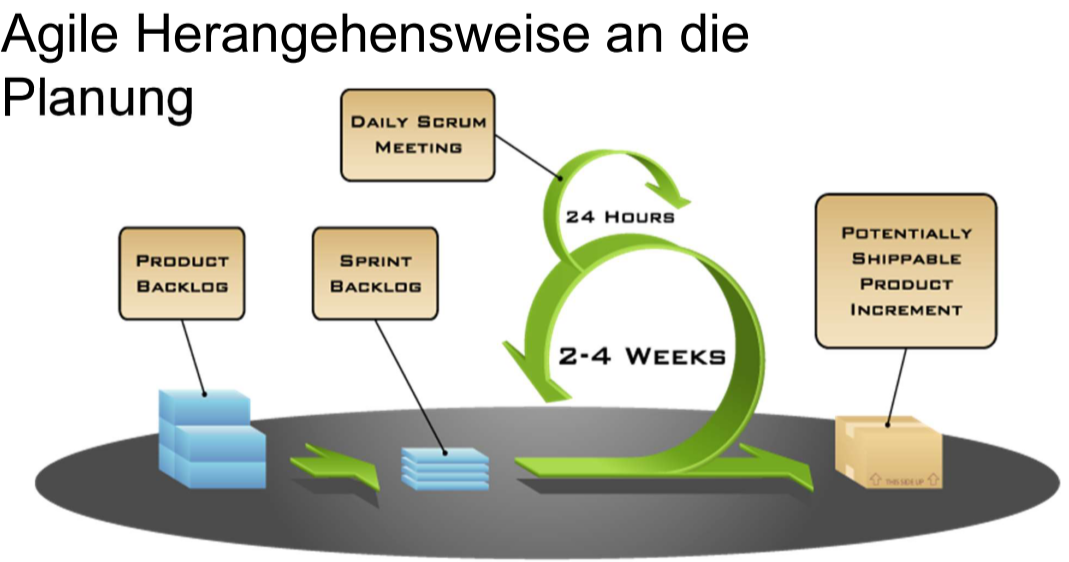
\includegraphics[width=400px]{img/HerangehensweiseAnDiePlanung.png}
	\captionof{figure}{Herangehensweise an die Planung}
	\label{fig:Herangehensweise an die Planung}
\end{Figure}

\section{der agile Ansatz}
\begin{itemize}
	\item grossartige Softwarte wird von grossartigen Individuen gebaut
	\item laufende Softwarte vor Dokumentation, weil dies frühes Feedback möglich macht
	\item Zusammenarbeit statt Verhandlung
	\item Auf Änderungen reagieren statt Plan folgen
\end{itemize}

Der agile Ansatz für die Planung:
\begin{itemize}
	\item Projekt erzeugt neue Fähigkeiten und neues Wissen in schneller Abfolge
	\item Neue Fähigkeit als Produkt geliefert
	\item neues Wissen ist die Basis
\end{itemize}

\section{Mehrere Planungsebenen}
Agile Teams planen auf mindestens drei Ebenen. Die Planungszwiebel sieht folgende Schichten voraus:
\begin{itemize}
	\item Strategy
	\item Portfolio
	\item Product
	\item Release
	\item Iteration
	\item Day
\end{itemize}

\section{Condition of Satisfaction}
Grundsätzlich wird jedes Projekt mit einer gewissen Menge von Zielen initialisiert. Dabei werden weitere Ziele bezüglich dem Zeitplan, Budget und der Qualität definiert. Diese Ziele sind für den Kunden oder Product Owner die \textbf{Condition of Satisfaction}. Die Condition of Satisfaction bestimmt die Planung der Releases und der Iterationen.

\section{Story Points}
Die Story Points bestimmen die Grösse einer Story, da dies für die Schätzung des Aufwands für das bestimmte Feature ist. Dabei ist ein Story Point eine relative Messung der Komplexität einer User Story.\\
Dabei ist die \textbf{Velocity} die Fortschrittsmessung eines Teams. Dies wird durch die Summe während einer Iteration umgesetzten Story Points, die jeder  User Story zugeordnet sind.

\section{Schätzen}
Die Schätzung sollte jeweils in Zusammenarbeit mit dem Team entstehen, hierzu eignet sich beispielsweise \textit{Planning Poker}. Da wir Menschen am besten mit einer Grössenordnung schätzen können, könnten wir beispielsweise die Fibonacci-Folge oder $2^n$ verwenden. 0 ist dabei keine gültige Schätzgrösse.\\
Eine grosse User-Story wird als \textbf{Epic} bezeichnet. Zusammenhängende Menge an User-Stories können zu einer Einheit gruppiert werden, dies wird dann \textbf{Theme} genannt.

\section{Planung von Releases und Iterationen}
\subsection{Release Plan}
Die Releaseplanung ist ein Prozess der einen Plang für 3-9 Monate und mehrere Iterationen umfasst. Es beschreibt was soll wann durch wen gebaut werden\\
\textbf{Release Plan auf einen Blick}:
\begin{itemize}
	\item 3-9 Monate
	\item priorisierte Liste von User-Stories mit mind. drei Schätzungen
	\item definiert Anzahl und Länge der Iterationen
	\item Priorisierung nach Conidition of Satisfaction
	\item Es sollte mit geschätzer und nachgebesserter Velocity gearbeitet werden
	\item Releaseplan wird zum Start jeder Iteration angepasst
\end{itemize}

\textit{Schritt 1 - \textbf{Definition der Condition of Satisfaction}:}\\
\begin{itemize}
	\item Die Kriterien müssen vor dem Planungsstart bekannt sein.
	\item Business Case ist hierzu häufig relevant (Wie viel Geld wird gespart / zusätzlich generiert)
	\item {Zeitplan, Scope und Ressourcen sind häufige Indikatoren
		\begin{itemize}
			\item Aus Sicht Product Owner sind die Condition of Satisfaction durch eine Kombination der INdikatoren gegeben
			\item \textit{date-driven} fixe Release-Zeitpunkte, variable Funktionalität
			\item \textit{feature-driven} Funktionalität wird höher bewertet als der Zeitplan
		\end{itemize}
	}
\end{itemize}

\textit{Schritt 2.1 - \textbf{Schätzung der User Stories}:}\\
\begin{itemize}
	\item Product Owner braucht Schätzung für alle Stories die im Vertrag enthalten sind
	\item Planung ist eine gemeinsame Tätigkeit
	\item zeitliche Schätzung wertvoll, wenn sie annähernd korrekt ist (plus/minus 20\%), jedoch wertlos ohne Bezug zur Realität
\end{itemize}

\textit{Schritt 2.2 - \textbf{Vorgehen für die Schätzung der User Stories}:}\\
\begin{itemize}
	\item Team muss schätzen nicht Product Owner
	\item nicht zu viel Zeit dafür aufwenden
	\item grobe Schätzung, keine festen Zusagen
\end{itemize}

\textit{Schritt 3A - \textbf{Bestimmen der Länge einer Iteration}:}\\
\begin{itemize}
	\item Länge ist meistens zwischen 2-4 Wochen
	\item Gibt gewisse Einflussfaktoren (Länge Releases, Unsicherheit, Prioritäten, etc.)
\end{itemize}

\textit{Schritt 3B - \textbf{Schätzung der Velocity}:}\\
\begin{itemize}
	\item Erfahrungswerte verwenden
	\item Eine Iteration durchlaufen (oder 2,3)
	\item {Einen Forecast erstellen
	\begin{itemize}
		\item Schätzung Anzahl Stunden pro Tag und Person im Projekt
		\item Berechnen der Anzahl Stunden pro Iteration
		\item Zufällige Auswahl von User Stories und Abbildung auf Tasks
	\end{itemize}
	}
\end{itemize}

\textit{Schritt 3C - \textbf{Priorisierung der User Stories}:}\\
Im Normalfall gibt es zu wenig Zeit für die Anzahl von Funktionen, aus diesem Grund muss der Product Owner entsprechend priorisieren. Schwellwerte für die Akzeptanz sind eine mögliche Art der Priorisierung.

\textit{Schritt 4 - \textbf{User Stories auswählen und Releasedatum festlegen}:}\\
Jetzt liegen Schätzungen und Velocity vor. Bei einem
\begin{itemize}
	\item \textbf{feature-driven Projekt}: Aufsummieren der Schätzungen aller Funktionen und teilen durch die erwartete Velocity $\rightarrow$ Release Date
	\item \textbf{date-Driven Projekt}: Multiplizieren der Anzahl Iteration mit der zu erwartenden Velocity $\rightarrow$ Anzahl Story Points pro Release
\end{itemize}
Nach jeder Iteration wird ein Update des Release Plans vorgenommen

\subsection{Iterationsplan}
Ist eine detaillierte Sicht auf die Arbeit während der Iteration. Wobei grössere User Stories in Tasks einer Iteration aufgeteilt werden. Jeder Task wird anhand Stunden geschätzt.

\section{Priorisierung}
Die Priorisierung setzt sich mit der Grundfrage ``Welche Funktionen sollten entwickelt werden?'' auseinander. Dabei sind folgende Faktoren relevant:\\
\begin{itemize}
	\item finanzielle Wert einer Funktion (wie viel Geld wird gespart / verdient)
	\item Kosten für die Entwicklung und Unterhalt (wieviele Story Points)
	\item Umfang
	\item Signifikanz des Know-how Gewinns
	\item Risiken als Konsequenz der Umsetzung einer Funktion (Zeitplan, Kosten und Risiken)
\end{itemize}

\subsection{Finanzielle Wert}
Priorisierung in Bezug auf den Business Value: Ersparnis oder zusätzliche Einnahmen durch eine bestimmte Funktion.\\
Werte der Zeit:\\
\textit{Net Present Value (NPV)}:
\begin{equation}
NPV(i) = \sum\limits^n_{t=0} F_t (1+i)^{-t}
\end{equation}
\textit{Return On Investment (ROI)}:
\begin{equation}
	0 = PV(i*) = \sum\limits^n_{t=0} F_t (1+i)^{-t}
\end{equation}

\subsection{Kosten}
Einer der wichtigsten Determinante für die Priorisierung. Oftmals wird übersehen, dass die Kosten sich über die Zeit verändern. Es sollte eine grobe Abbildung von Story Points / Tage in Geld erfolgen.

\subsection{Neues Wissen}
Häufig wird ein guter Teil des Aufwandes  für neues Wissen aufgewendet. Dieser Aufwand muss als fundamental für das Projekt anerkannt werden. Dabei unterscheidet man zwischen \textit{Was wird entwickelt} $\rightarrow$ Wissen über das Produkt und \textit{Wie wird entwickelt} $\rightarrow$ Wissen über das Projekt.

\subsection{Risiken}
Risiken sind ein wichtiger Bestand eines Projektes und haben eine gewisse Eintretenswahrscheinlichkeit und einen Impact auf das Projekt, falls diese eintreten. Es gibt:\\
\begin{itemize}
	\item zeitliche Risiken
	\item Risiken bezüglich Kosten
	\item funktionale Risiken
\end{itemize}

\section{Tracking}
\subsection{Überwachung Release Plan}
Der \textit{Release-Plan} wird mit einem \textbf{Burndown-Chart} überwacht.
\begin{itemize}
	\item Wenn die Arbeit abgeschlossen ist, wird der Balken nach unten korrigiert
	\item Bei Korrekturen wird der Balken nach oben oder unten korrigiert
	\item Bei neuen Arbeiten wird der Boden des Balken gesenkt
	\item Beim entfernen von Arbeiten wird der Boden des Balken angehoben
\end{itemize}

Die \textbf{Parking-Lot Chart} zeigt wie viel eines Themes (Sammlung von User-Stories) bereits realisiert wurden

\subsection{Überwachung Iteration Plan}
Der Iterationsplan wird entweder mit einem \textbf{Task Board} oder einem \textbf{Iteration Burndown Chart} überwacht

\chapter{Version Control}

\section{ITIL}
ITIL steht für \textbf{IT Infrastrcucture Library} und ist eine Sammlung von Best Practice Prozessen, die für den Betrieb einer IT Infrastruktur notwendig sind.

\begin{Figure}
\centering
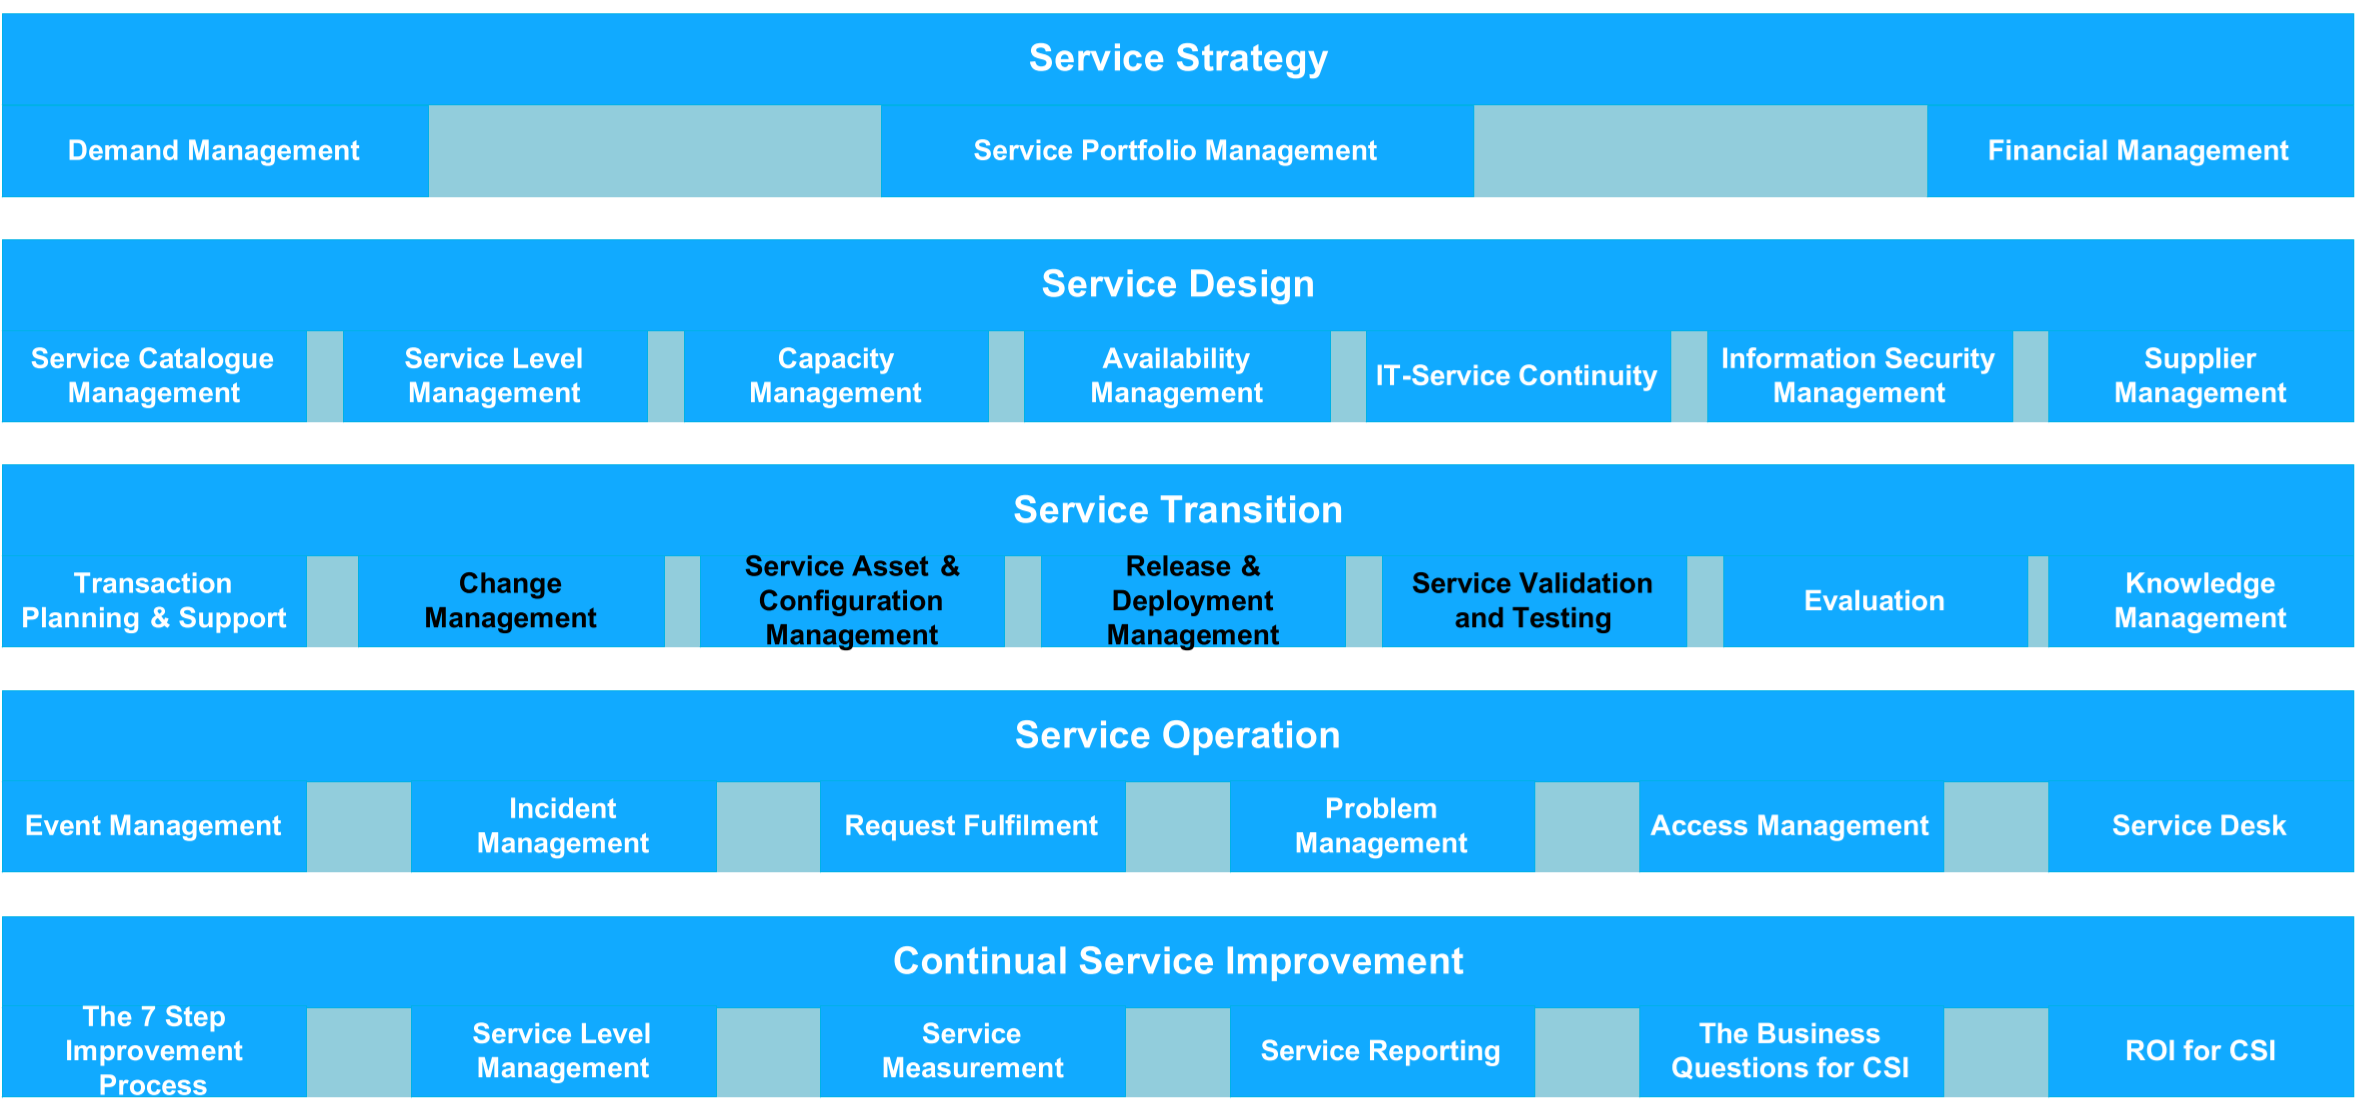
\includegraphics[width=400px]{img/itilLifecycle.png}
	\captionof{figure}{Abbildung des ITIL-Lifecycles}
	\label{fig:ITIL Lifecycle}
\end{Figure}

\begin{Figure}
\centering
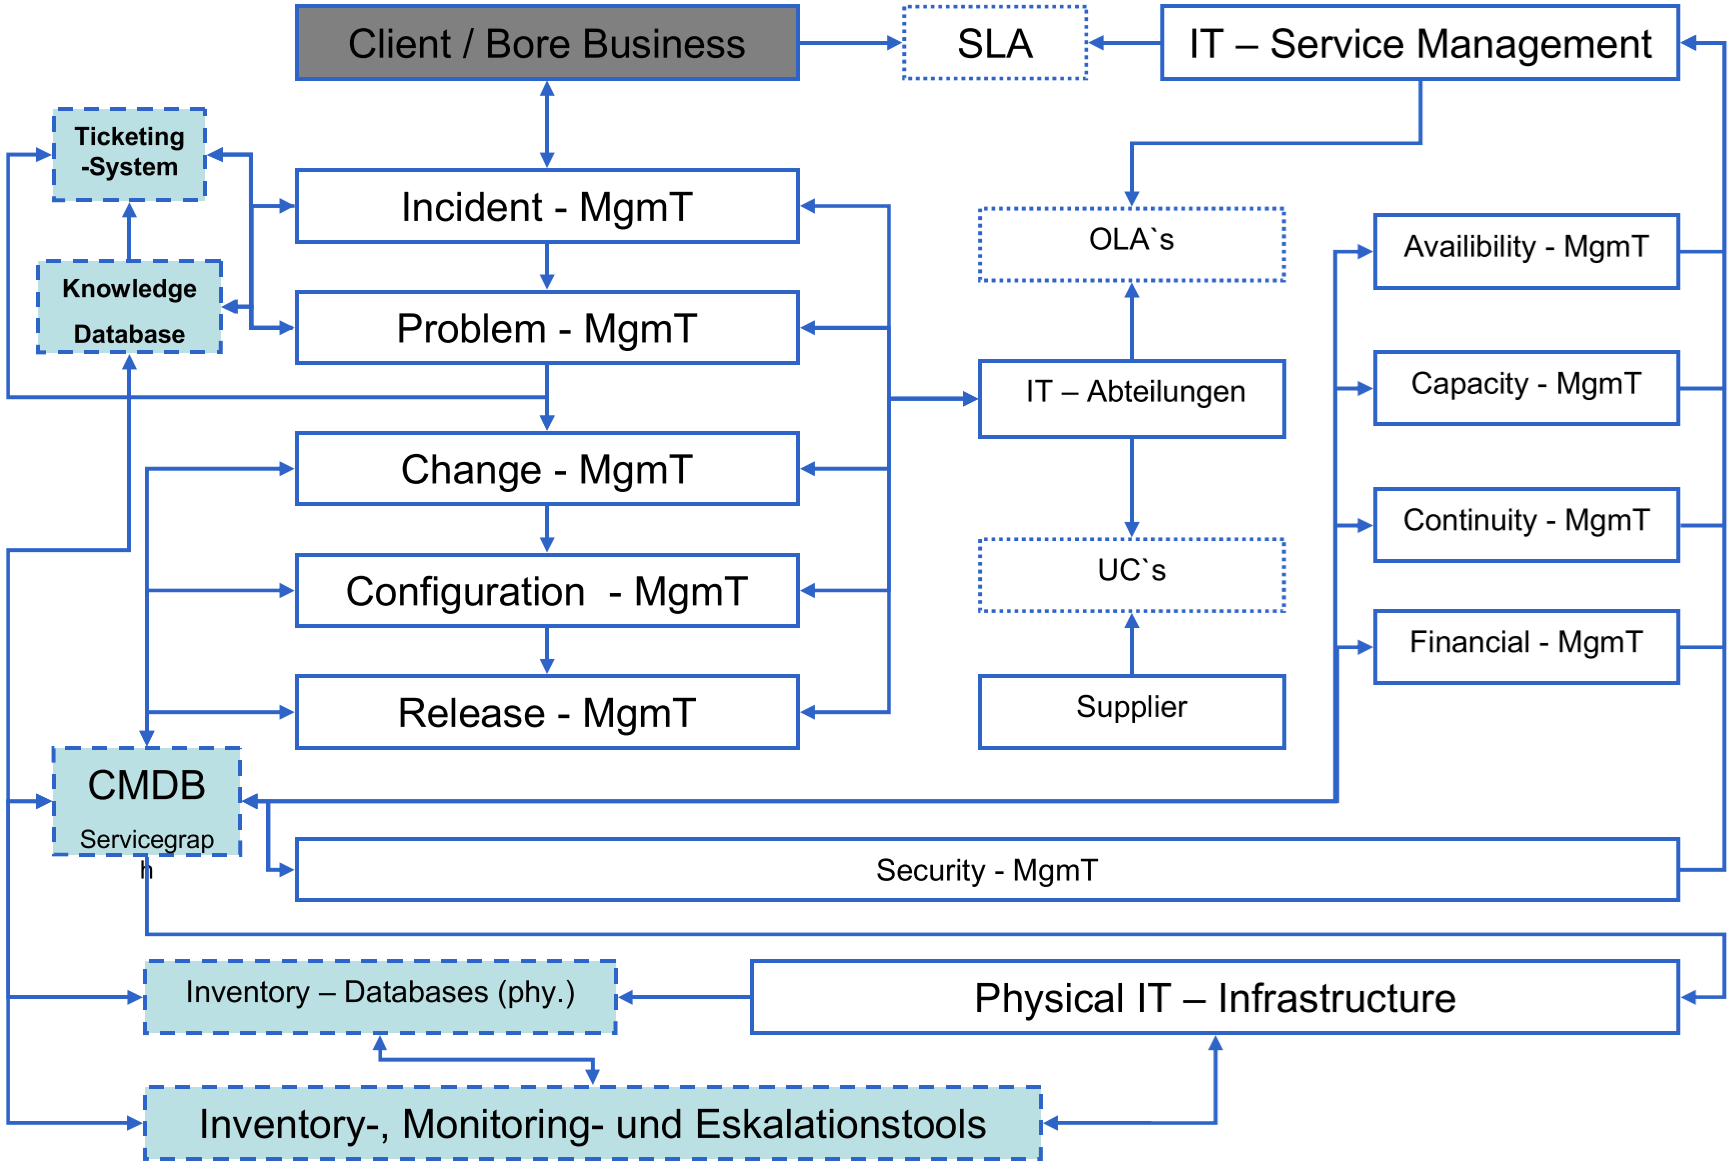
\includegraphics[width=400px]{img/itilProzesse.png}
	\captionof{figure}{Abbildung der ITIL-Prozesse}
	\label{fig:ITIL Prozesse}
\end{Figure}

\textbf{Incident Management}:\\
Prozesse zur Umsetzung von Anfragen, Kundenbedürfnissen oder Meldungen über Servicebeeintraächtigungen. Incident Management = First Level Support $\rightarrow$ meist Service Desk oder Call Center\\

\textbf{Problem Management}: \\
Löst Probleme schnell und wirksam. Probleme sind Incidents die keine Änderung der Konfiguration oder Software erfordern. Problem Management = Second Level Support $\rightarrow$ meist durch System-Spezialisten\\

\textbf{Change Management}:\\
stellt sich, dass alle notwendigen Änderungen in einem System gut vorbereitet und kontrolliert ablaufen. Gemäss Dr. Jacky Estublier \textit{Software Configuration Management bedeutet die Kontrolle der Evolution komplexer Systeme} Die Definition in der OO-Welt sieht wie folgt aus: \textit{Configuration Management- The task of defining and maintaining configurations and versions of artifacts. This includes baselining, version control, status control and storage control of the artifacts}. \\
Die Grundproblematik:\\
\begin{itemize}
	\item \textbf{Programming in the Large} $\rightarrow$ Versionierung, Rebuilding, Zusammenstellung (Composition)
	\item \textbf{Programming in the Many} $\rightarrow$ Prozessunterstützung, concurrent Engineering
	\item \textbf{Programming in the Wide} $\rightarrow$ Web Remote Engineering
\end{itemize}

Die Grundbegriffe:\\
\begin{itemize}
	\item \textbf{Configuration Item} $\rightarrow$ Ansammlung von Hardware, Software oder beidem, ist dazu bestimmt das einzelne mittels Configuration Management zu verwalten
	\item \textbf{Baseline} $\rightarrow$ Spezifikation oder Produkt, welches auf formale Art begutachtet wird. Baseline kann durch formalen Change Prozess verändert werden.
	\item \textbf{Release} $\rightarrow$ Version, welche abgeschlossen und dessen Entwicklungsprozess abgeschlossen ist. Release ist öffentlich zugänglich.
	\item \textbf{Version} $\rightarrow$ bestimmte, normalerweise nummerierte Ausprägung einer Spezifikation oder Produkt
	\item \textbf{Dependency} $\rightarrow$ Abhängigkeit zwischen einem oder mehreren Configuration Items


\end{itemize}

\textbf{Configuration Management}:\\
Identifikation, Überwachung, Statusnachweis und Verfikation sämtlicher in einem System verwendeten Komponenten zuständig.\\

\begin{Figure}
\centering
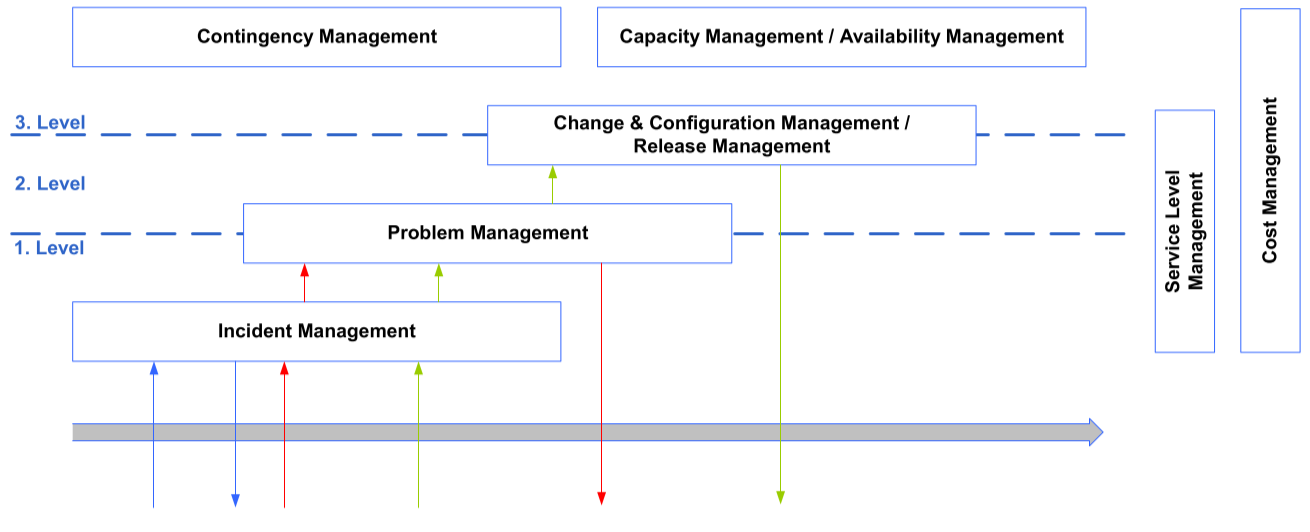
\includegraphics[width=400px]{img/itilLevelUebersicht.png}
	\captionof{figure}{Abbildung der Levels in ITIL}
	\label{fig:ITIL Level}
\end{Figure}

\textbf{Release Management}:\\
Für Planung, Dokumentation, Abnahme und Durchführung von Releases verantwortlich. Ein Release ist ein definiertes Set von Configuration Items, die im Rahmen des Configuration Managements verwaltet werden.\\

\textbf{Contigency Management}:\\
Contingency Planning (auch Eventualfall-Planung) bereits sich für den Eventualfall vor und um aus den vorhandenen Möglichkeiten die beste Lösung auszuwählen.\\

\textbf{Capacity Management}:\\
Die Kundeanforderungen sollen in Bezug auf Transaktionsvolumen, Durchlaufzeit und Antwortzeit erfüllt werden.\\

\textbf{Availability Management}:\\
Die IT-Infrastruktur ist mit einer definierten und überwachten Verfügbarkeit für Kunden zugänglich.\\

\textbf{Service Level Management}:\\
Steuerung der IT-Servicequalität durch das Erstellen eines Servicekatalogs, sowie Abschluss und Kontrolle von SLA's\\

\textbf{Cost Management}:\\
Kostenermittlung und Leistungsverrechnung von IT-Dienstleistungen

\begin{Figure}
\centering
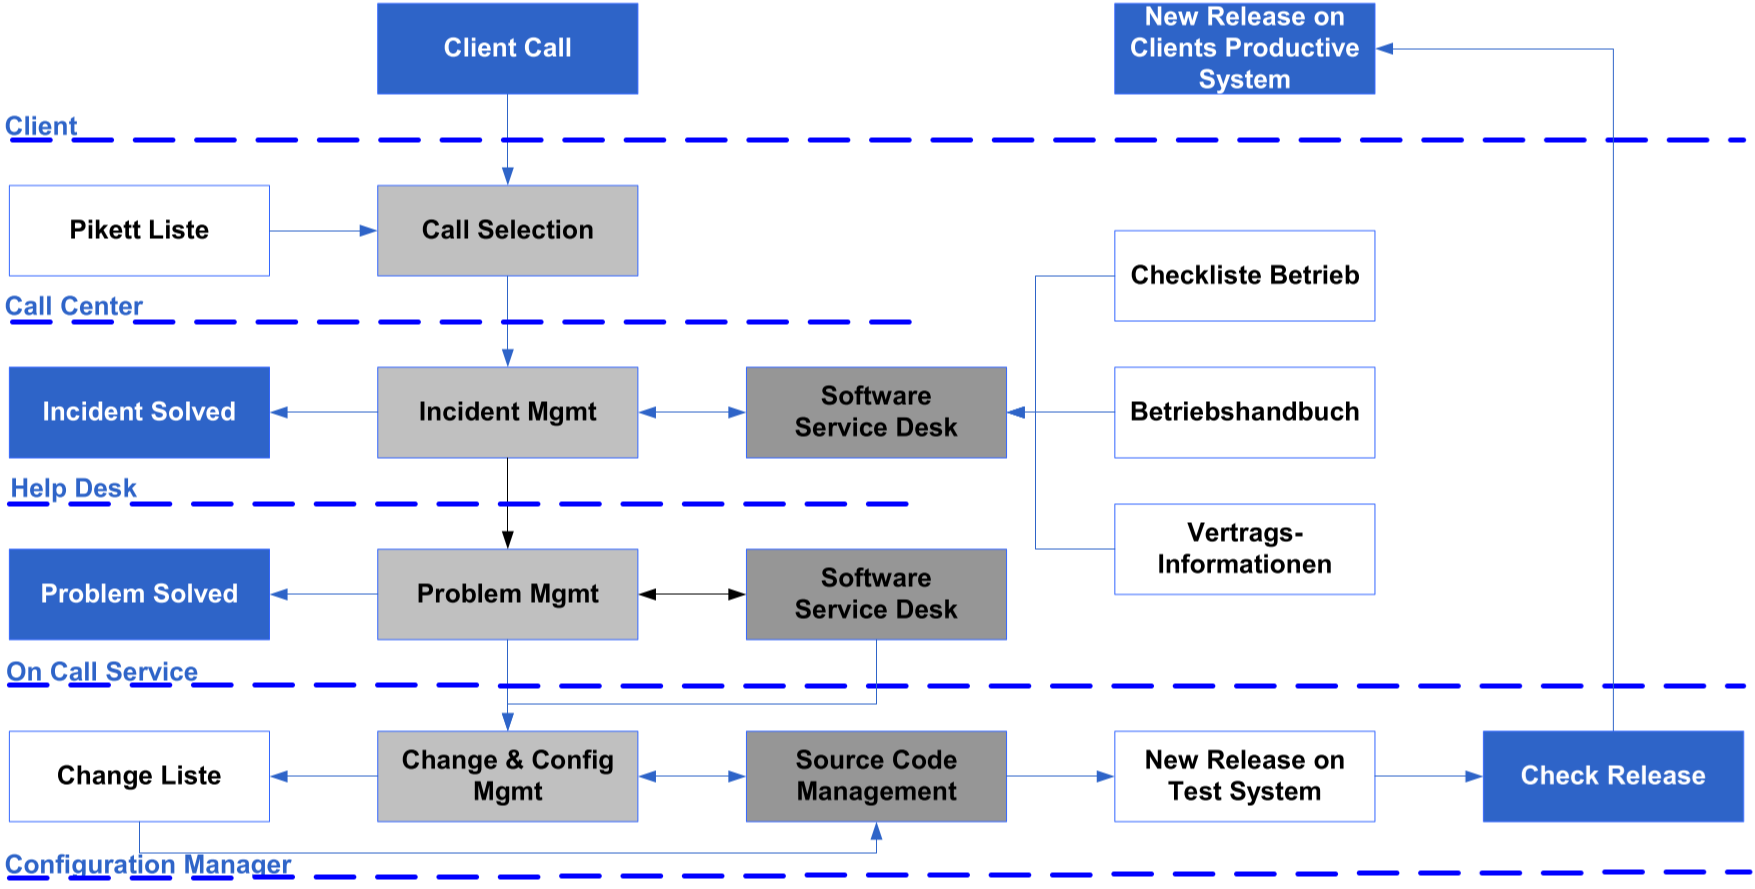
\includegraphics[width=400px]{img/Change.png}
	\captionof{figure}{Was führt zu einem Change}
	\label{fig:Was führt zu einem Change}
\end{Figure}


\chapter{Build Automation}

\section{Einführung DevOps}
Das Ziel von DevOps ist, zwei Sichtweisen (Entwicklung und Betrieb) zusammenzubringen.\\
Entwicklung:
\begin{itemize}
	\item sieht Entwicklung von Innen nach Aussen
	\item definiert Struktur, die aufgrund der Anforderungen gegeben ist
\end{itemize}
Betrieb:
\begin{itemize}
	\item sieht die Anwendung von Aussen nach Innen
	\item sieht die Anwendung als weiteres Element, dass verwaltet werden muss und am Leben erhalten werden soll
	\item definiert Struktur durch Betriebsumgebung
\end{itemize}

\section{Konzepte}
DevOps entstand aus der agilen Entwicklung. Das wichtigste Ziel ist die End-To-End Software Delivery Lifecycle und dabei soll die Entwicklung die produktive Infrastruktur besser verstehen.\\
Häufige \textbf{Herausforderungen} waren:\\
\begin{itemize}
	\item Entwicklung beachtet Rahmenbedingungen des Betriebs zu wenig
	\item Betrieb beachtet Geschäftszweck und den Wert der Software zu wenig
\end{itemize}

\textbf{Ziele von DevOps}:
\begin{itemize}
	\item Erhöhung Deployment Frequenz
	\item Schnelleres Time to Market
	\item Niedrigere Fehlerrate für neue Releases
	\item kürzere Fehlerbehebungszeit
	\item Verbesserung der MTTR (mean time to recovery) - Wiederherstellugnszeit
\end{itemize}

\textbf{DevOps Einführungsstufen}:
\begin{enumerate}
	\item Lieferung im Wasserfallmodell
	\item Continuous Integration
	\item Continuous Delivery
	\item Continuous Deployment
\end{enumerate}

\textbf{Werte}:
\begin{itemize}
	\item DevOps Kultur = Verbesserung Zusammenarbeit
	\item Abnahme Silo-Denken
	\item Geteilte Verantwortung
	\item Autonome Teams
	\item Verbesserte Qualität
	\item Wertendes Feedback
	\item Erhöhung Automation
\end{itemize}

\textbf{Tools}:
\begin{itemize}
	\item Source Code Repository
	\item Build Server
	\item Configuration Management
	\item Virtual Infrastructure
	\item Test Automation
	\item Pipeline Orchestration
	\item Unifying Enterprise Software Devolopment and Delivery
\end{itemize}

\section{Grundlegende Problematik}

\begin{Figure}
\centering
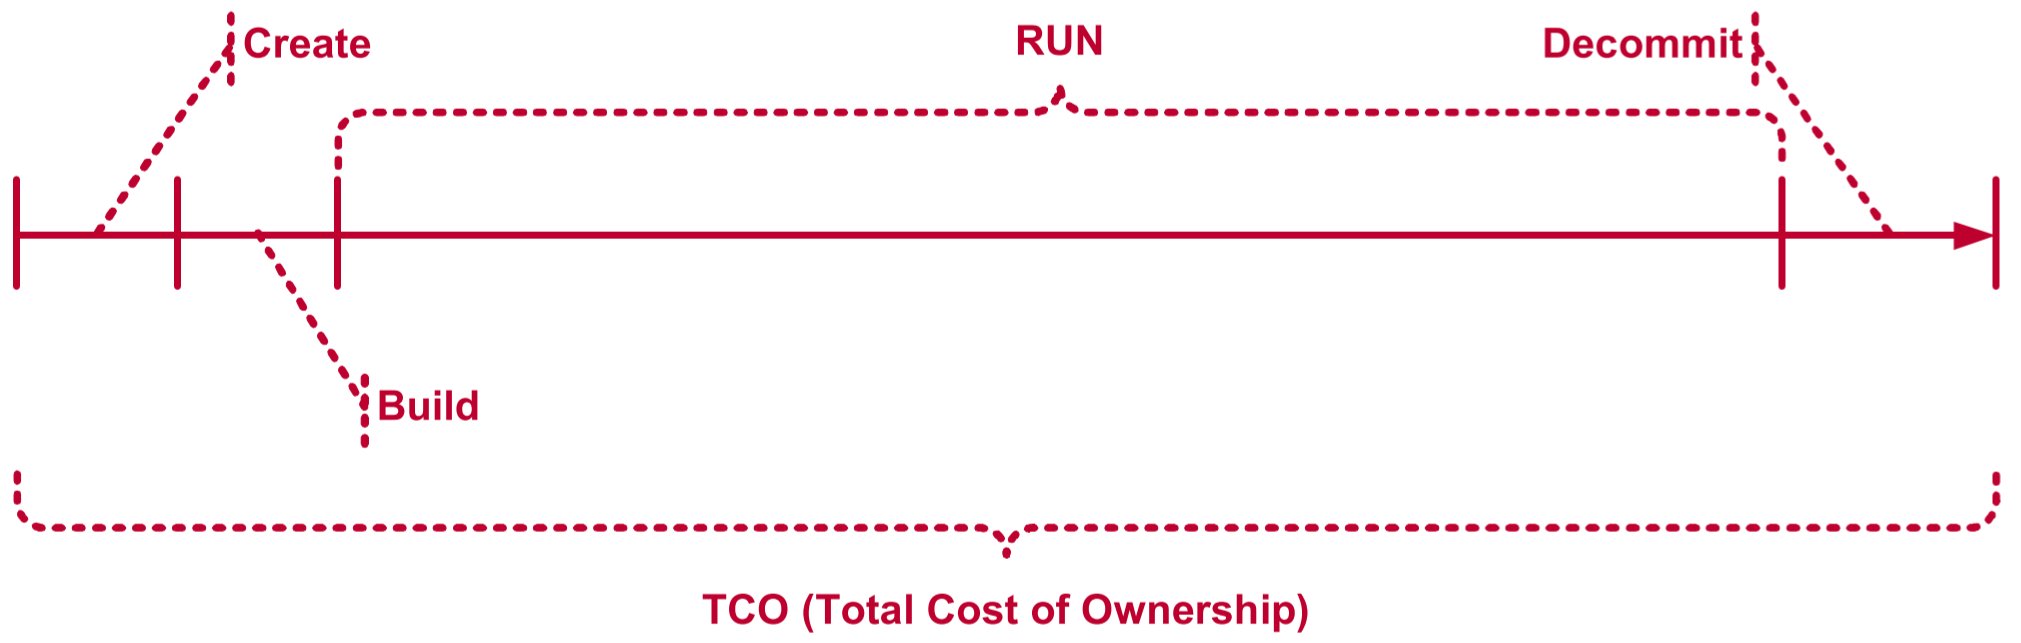
\includegraphics[width=400px]{img/RelationDevOps.png}
	\captionof{figure}{Die Relation zwischen Dev - Ops}
	\label{fig:Die Relation zwischen Dev - Ops}
\end{Figure}

Tatsachen:
\begin{itemize}
	\item Unterhaltskosten sind ca 20\% der Entwicklungskosten
	\item 39\% aller Fehler sind Schnittstellenfehler ($\rightarrow$ und werden oft erst spat im Entwicklungsprozess entdeckt
	\item nur wenige Releases enden ohne Fehlersituationen
	\item gute Testdaten sind immer ein Problem
	\item Ausbau von Logging und Tracing ist nicht immer eine Lösung
	\item nicht funktionale Eigenschaften werden erst im Betrieb sichtbar
\end{itemize}

\section{Wirtschaftliche Vorteile}
\begin{itemize}
	\item \textbf{schnellere Umsetzung}: Mehr als doppelt so schnelle Umsetzung von Changes / Fixes
	\item \textbf{weniger Fehler}: 3 mal weniger Fehler bei der Einführung von Changes
	\item \textbf{höhere Stabilität der Systeme}: 24 mal schnellere Wiederherstellungszeit
	\item \textbf{Verbesserte Produktivität}: Erhöhung der Produktivtät von Entwicklung und Betrieb um knapp 30\%
\end{itemize}

\section{DevOps Elemente}
\begin{Figure}
\centering
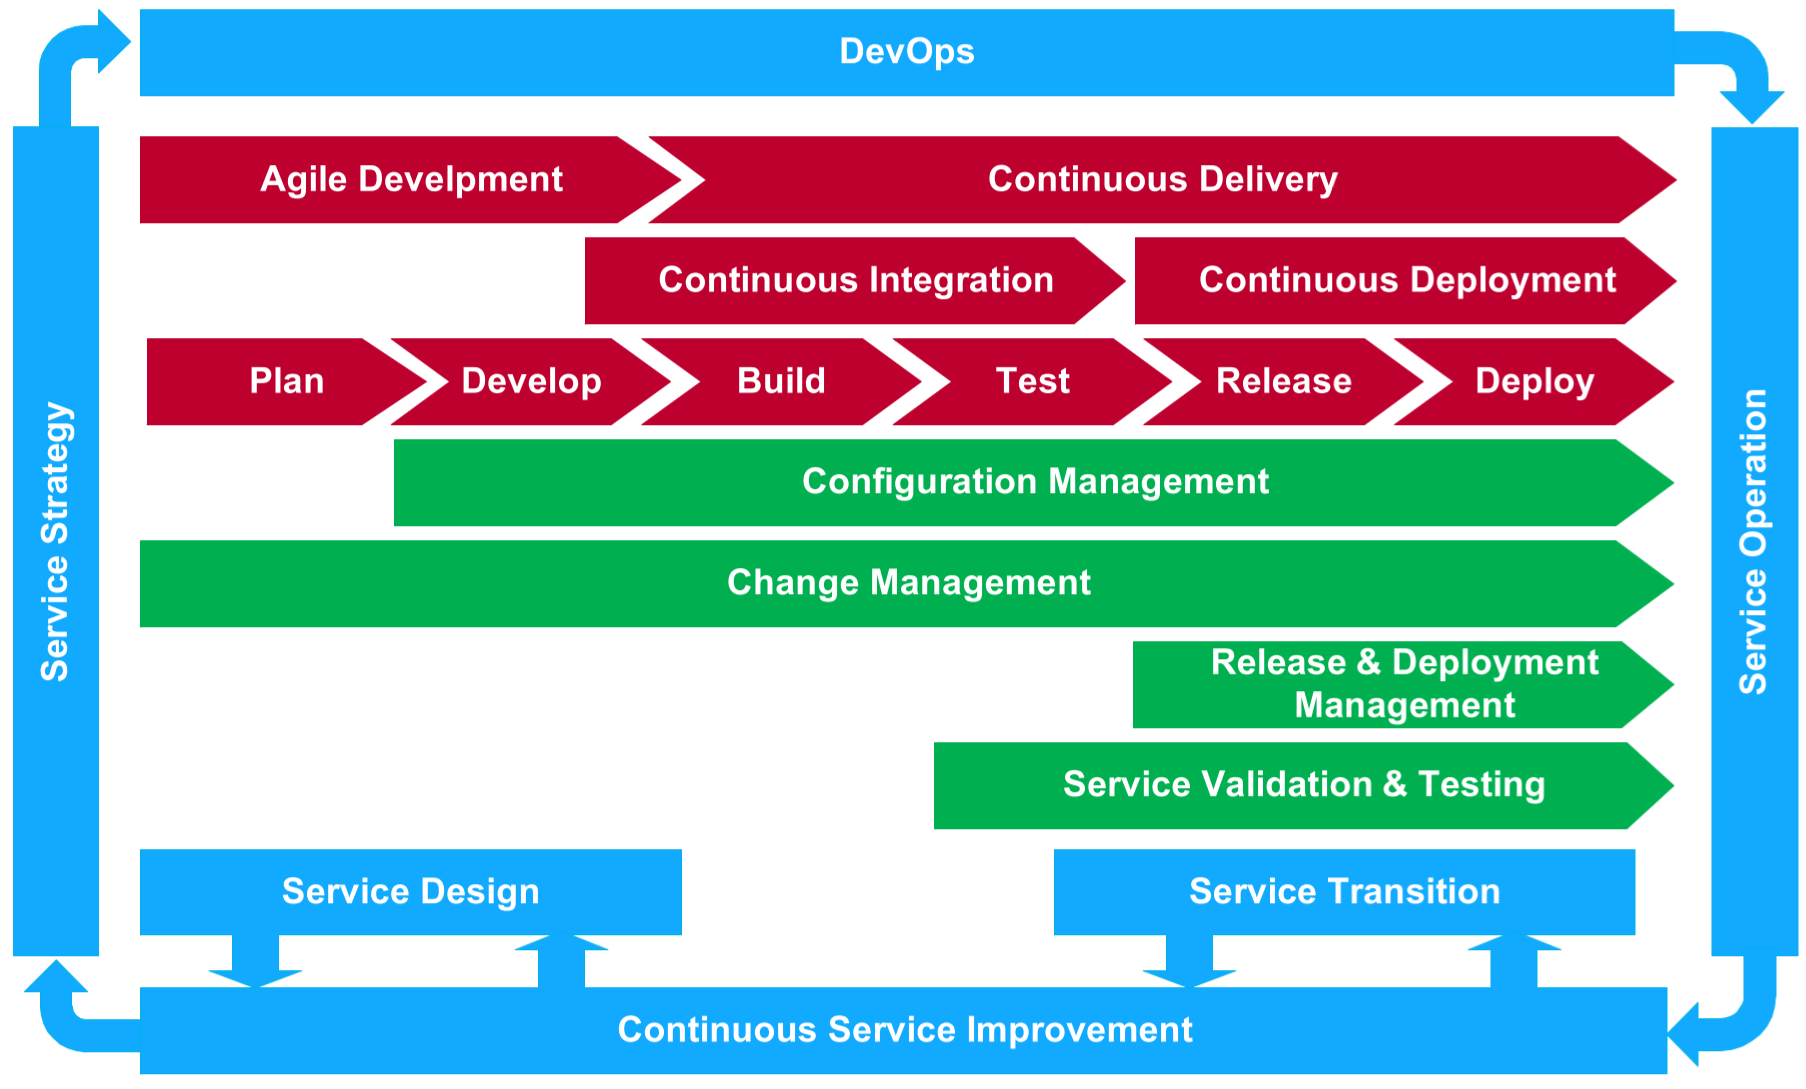
\includegraphics[width=400px]{img/DevOpsElemente.png}
	\captionof{figure}{Die Relation zwischen Dev - Ops}
	\label{fig:Die Relation zwischen Dev - Ops}
\end{Figure}

\subsection{Die DEV Elemente}
\begin{itemize}
	\item \textbf{Agile Development} $\rightarrow$ Entwicklungsmethodik mit Fokus auf lauffähige Softwarte, kleiner Schritte zusammen mit Kunden
	\item \textbf{Continuous Integration} $\rightarrow$ Automatisiertes und schneller bereitstellen und testen lauffähiger Software
	\item \textbf{Continuous Deployment} $\rightarrow$ Jede Änderung geht sofort in Produktion, um schnelles Feedback zu gewährleisten
	\item \textbf{Continuous Delivery} $\rightarrow$ Durchgänge Automatisierung von der Bereitstellung über das Testen bis hin zur Auslieferung in die Produktion
	\item \textbf{Plan} $\rightarrow$ Planung der Umsetzung bestimmter Produkteigenschaften
	\item \textbf{Develop} $\rightarrow$ Entwicklung
	\item \textbf{Build} $\rightarrow$ Zusammenstellung einer lauffähigen und testbaren Produktversion
	\item \textbf{Test} $\rightarrow$ Testen
	\item \textbf{Release} $\rightarrow$ Zusammenstellung einer vollständig lauffähigen Produktversion
	\item \textbf{Deploy} $\rightarrow$ Bereitstellung der Produktversion in eine Laufzeitumgebung

\end{itemize}

\subsubsection{10 Dev-Agile Gebote}
\begin{enumerate}
	\item aktiver Einbezug des Kunden
	\item Team muss Entscheidungen treffen können
	\item Anforderungen verändern sich, der zeitliche Ablauf ist fix
	\item Anforderungen sind auf hoher Ebene zu erfassen; leichtgewicht und visuell
	\item Es sind kleine, inkrementelle Releases iterative zu Entwickeln
	\item Konzentration auf häufige Auslieferungen von Produkten
	\item Fertigstellung einer bestimmten funktionalen Einheit vor der Umsetzung des Nächsten
	\item gilt 80 / 20 Regel
	\item Testen ist ein integraler Bestandteil des Projekt-Lebenszyklus - früh und oft testen
	\item gemeinschaftlicher und partnerschaftlicher Ansatz zwischen allen Stakeholdern
\end{enumerate}

\subsubsection{DEV - Continuous}
\textbf{Continuous Integration}
\begin{itemize}
	\item tägliches Check-In während der Entwicklung
	\item Automatisierte Erstellung einer lauffähigen Version (build)
	\item Automatisierte Ausführung von Unit Tests
	\item Öffentlicher Zugriff auf die Testergebnisse
	\item Sehr schnelle Erstellung (build)
	\item Tests werden in einer Testumgegbung ausgeführt
\end{itemize}

\textbf{Continuous Deployment}
\begin{itemize}
	\item Jede Änderung geht direkt in die Produktion
	\item Neue Funktionalität wird durch sogenannte Feature Toggles nur eingeschränkter Nutzergruppe zur Verfügung gestellt
	\item schnelles Feedback
\end{itemize}

\textbf{Continuous Delivery}
\begin{itemize}
	\item Continuous Integration und Continuous Deployment
	\item Automatisierung der Regressionstests
	\item Vereinfachung der Freigabe durch automatisierte Freigabemechanismen
\end{itemize}

\subsection{Die OPS Elemente}

\begin{itemize}
	\item \textbf{Configuration Management} $\rightarrow$ Identifikation, Überwachung, Statusnachweis und Verfikation aller Systemkomponenten
	\item \textbf{Change Management} $\rightarrow$ Sicherstellung des gut vorbereiteten und kontrollierten Ablauf aller notwendigen Systemänderungen
	\item \textbf{Release und Deployment Management} $\rightarrow$ Planung, Dokumentation, Abnahme und die Durchführung von Releases
	\item \textbf{Service Strategy} $\rightarrow$ Business IT-Alginment für die IT-Service Bereitstellung
	\item \textbf{Service Design} $\rightarrow$ Gestaltung von IT-Services aufgrund von Anforderungen
	\item \textbf{Service Transition} $\rightarrow$ Aufbau und Rollout von IT-Services
	\item \textbf{Service Operations} $\rightarrow$ Betrieb von IT-Services
	\item \textbf{Continuous Service Improvement} $\rightarrow$ QSMethodik zur ständigen Verbesserung (gemäss ISO 20000)
\end{itemize}
\begin{Figure}
\centering
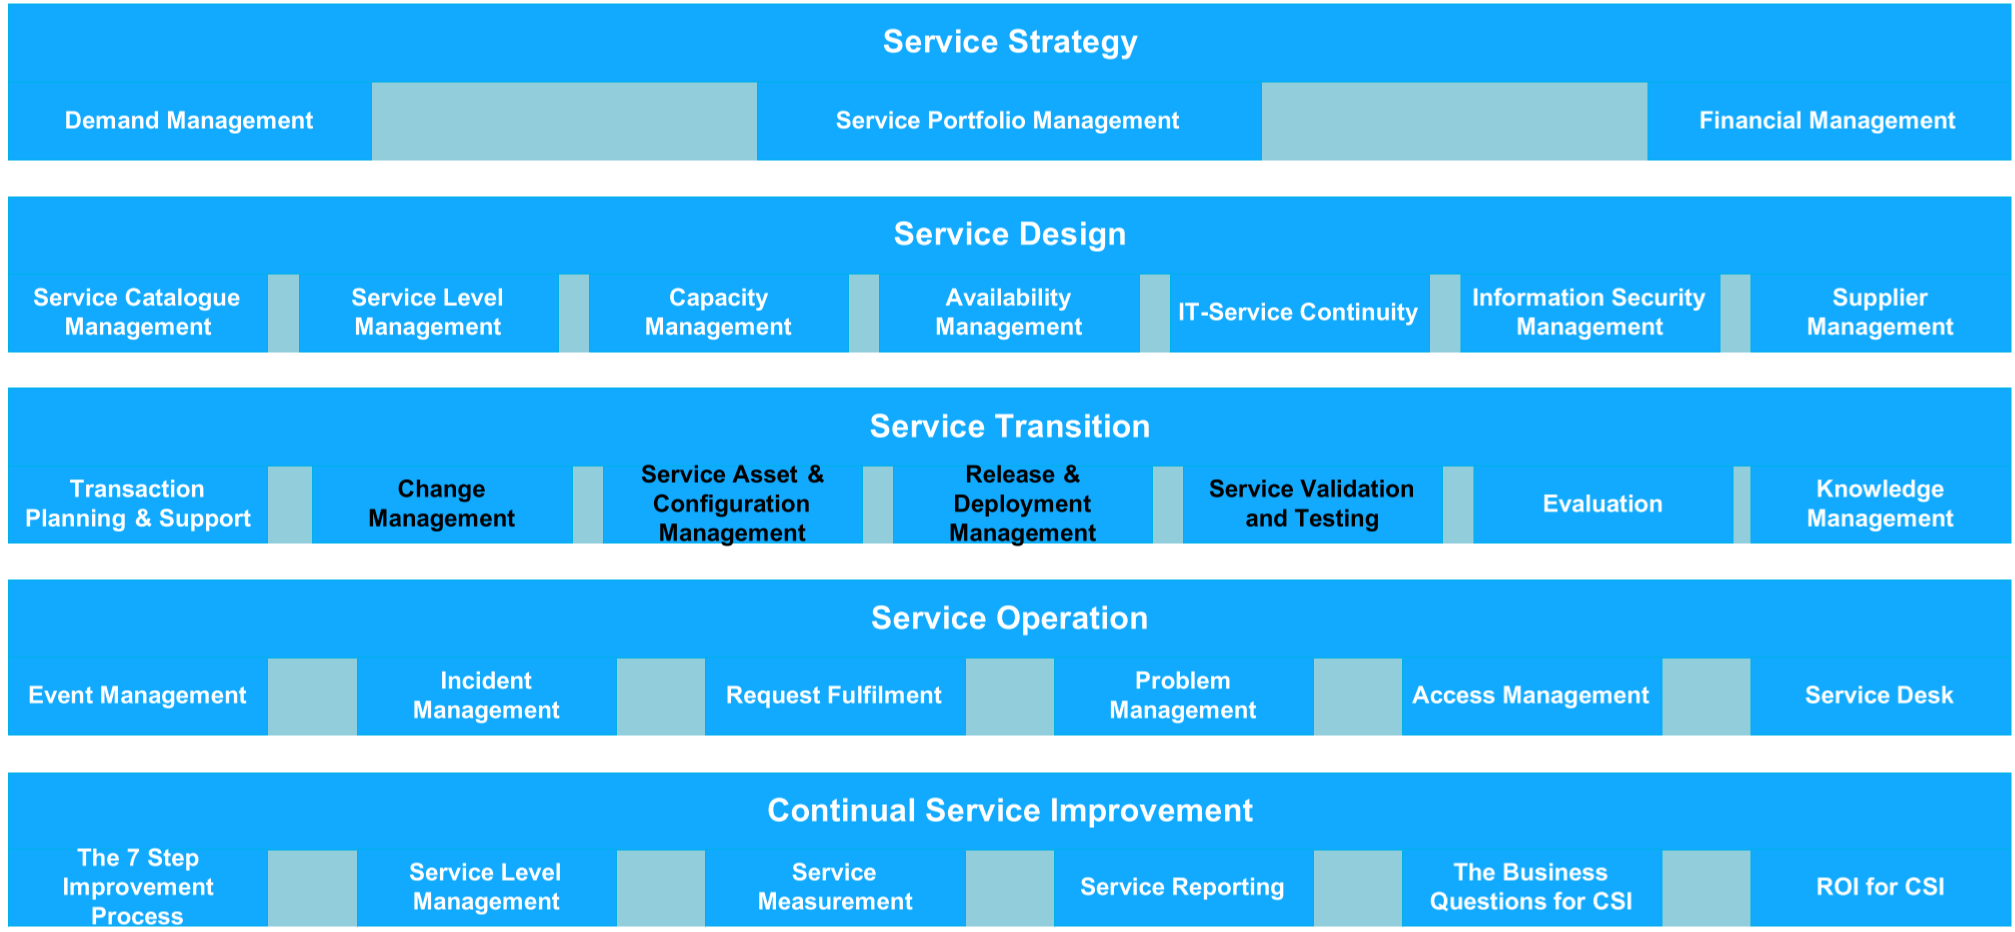
\includegraphics[width=400px]{img/ITILOps.png}
	\captionof{figure}{OPS Elemente gemäss ITIL}
	\label{fig:OPS Elemente gemäss ITIL}
\end{Figure}

\chapter{SCRUM}

\section{Ansatz}
\begin{itemize}
	\item Scrum ist ein agiler Prozess, welcher es erlaubt sich auf die Lieferung des \textbf{höchst mögliche Wertbeitrages für das Fach} zu konzentrieren
	\item Es erlaubt die rasche und wiederholte Inspektion des \textbf{aktuellen} Standes der \textbf{lauffähigen Software}
	\item \textbf{Das Fach setzt die Prioritäten}, des Teams \textbf{organiseren sich selbst}, um den besten Weg zu finden, die am höchsten priorisierten Funktionen zu liefern
	\item Jede 2-4 Wochen können alle Beteiligten \textbf{lauffähige Software} sehen und darüber entscheiden, ob ein Release freigegeben wird oder ob er ausgebaut werden soll
\end{itemize}

\section{Eigenschaften}
\begin{itemize}
	\item Selbstorganisierte Teams
	\item Produktfortschritt als Serie von 'Sprints' in Monats-Rhythmus
	\item Anforderungen werden in einem Backlog erfasst
	\item keine speziellen Engineering Vorgehen definiert
	\item Verwendet sich entwickelnde Regeln um eine agile Umgebung für die Lieferung von Projektergebnisse zu kreieren
	\item einer der agilen Prozesse
\end{itemize}

\textbf{Erinnerung agile Manifesto}
\begin{itemize}
	\item Individuen und Interaktion sind wichtiger als Prozessen und Tools
	\item Lauffähige Software ist wichtiger als durchgängige Dokumentation
	\item Zusammenarbeit mit dem Kunden ist wichtiger als Vertragsverhandlungen
	\item Auf Veränderungen reagieren ist wichtiger als einem Plan folgen
\end{itemize}

\subsubsection{Projekte und ihre Dynamik}
\begin{Figure}
\centering
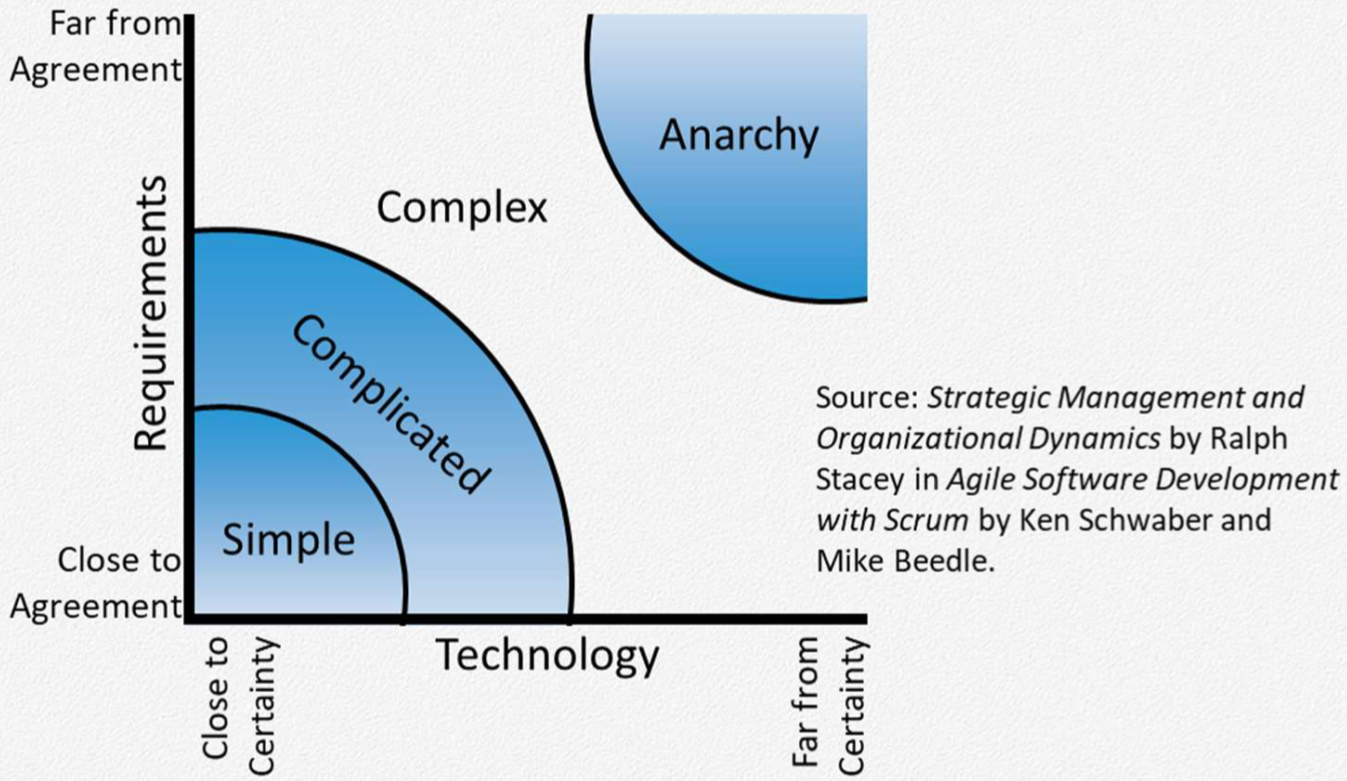
\includegraphics[width=400px]{img/Projektdynamik.png}
	\captionof{figure}{Projekte und ihre Dynamik}
	\label{fig:Projekte und ihre Dynamik}
\end{Figure}

Das Level der Projektdynamik lässt theoretisch auf zwei Ansätze aufzeigen:
\begin{itemize}
	\item Das \textbf{definierte} Prozesskontrollmodell: Einfache Prozesse mit wenig Dynamik, wiederholbar
	\item Das \textbf{empirische} Prozesskontrollmodell: Komplexe Prozesse mit viel Dynamik, nicht wiederholbar
\end{itemize}
Jedoch können die wenigsten Projekt mit einer der beiden Modellen gemanaged werden $\rightarrow$ Das empirische Modell mit regelmässigen Inspektionen und adaptiver Kontrolle ist anzuwenden

\section{SCRUM auf einen Blick}
\textit{How it fits}
\begin{Figure}
\centering
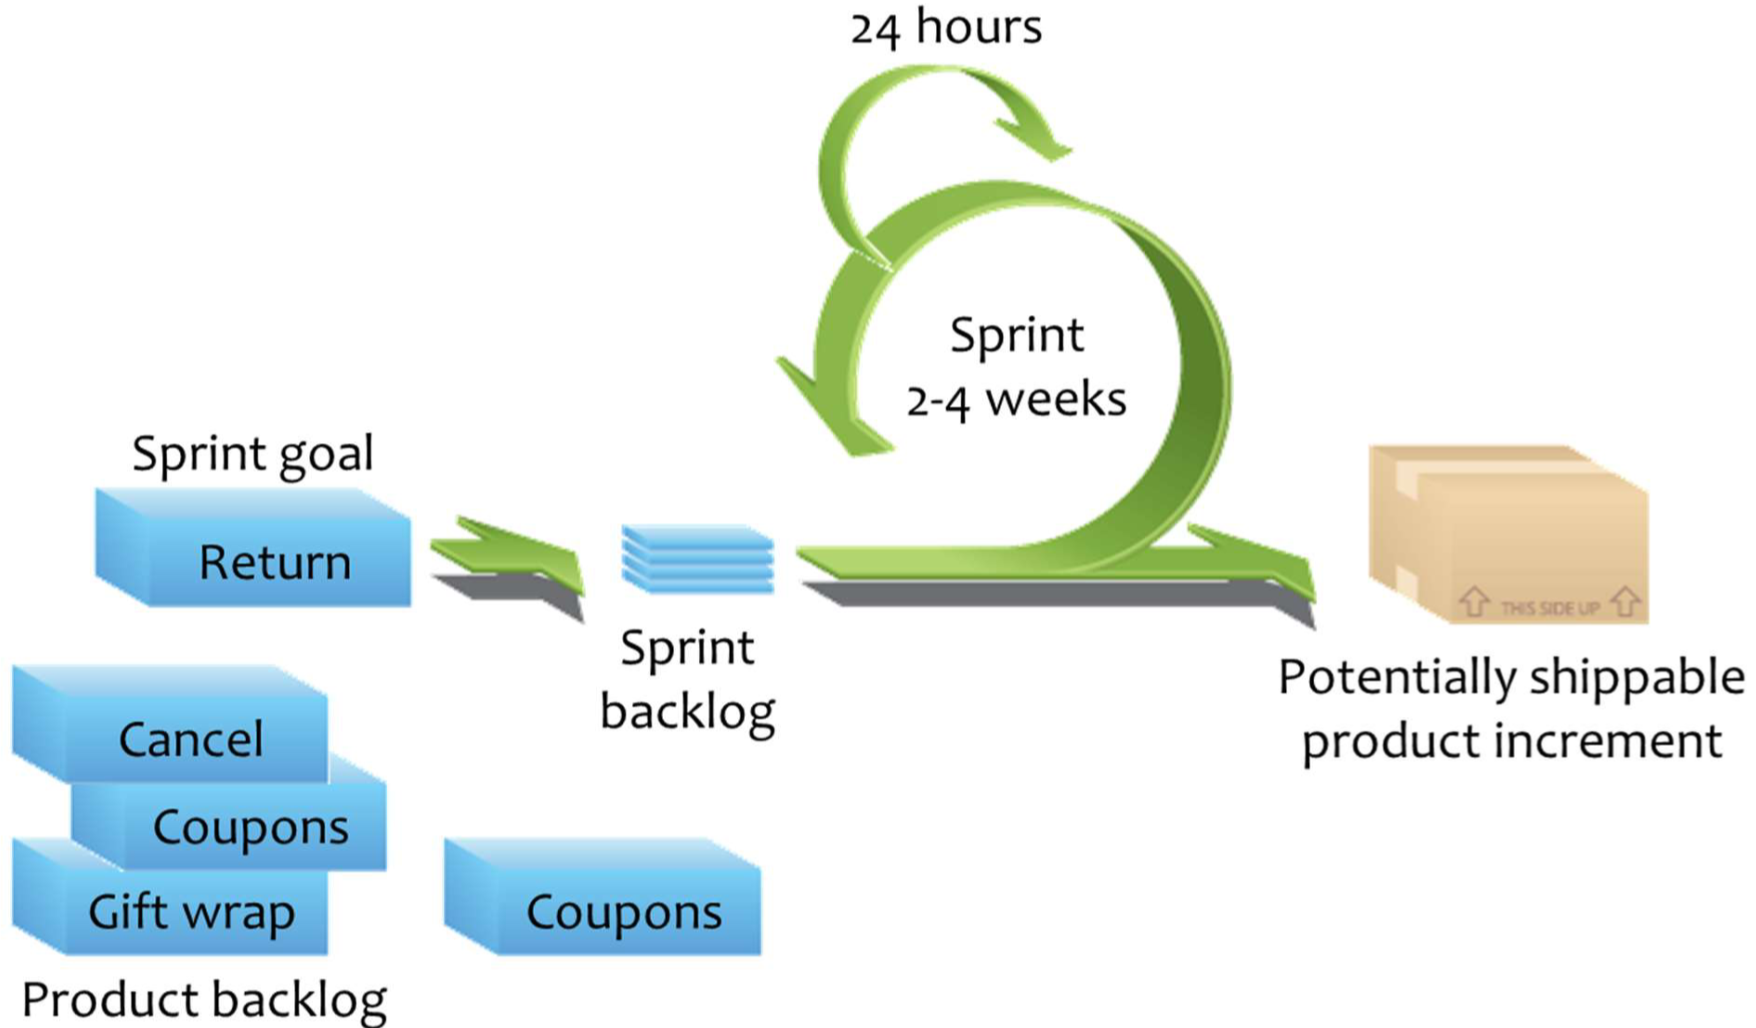
\includegraphics[width=400px]{img/HowScrumFits.png}
	\captionof{figure}{How Scrum fits}
	\label{fig:How Scrum fits}
\end{Figure}

\textit{How it works}
\begin{Figure}
\centering
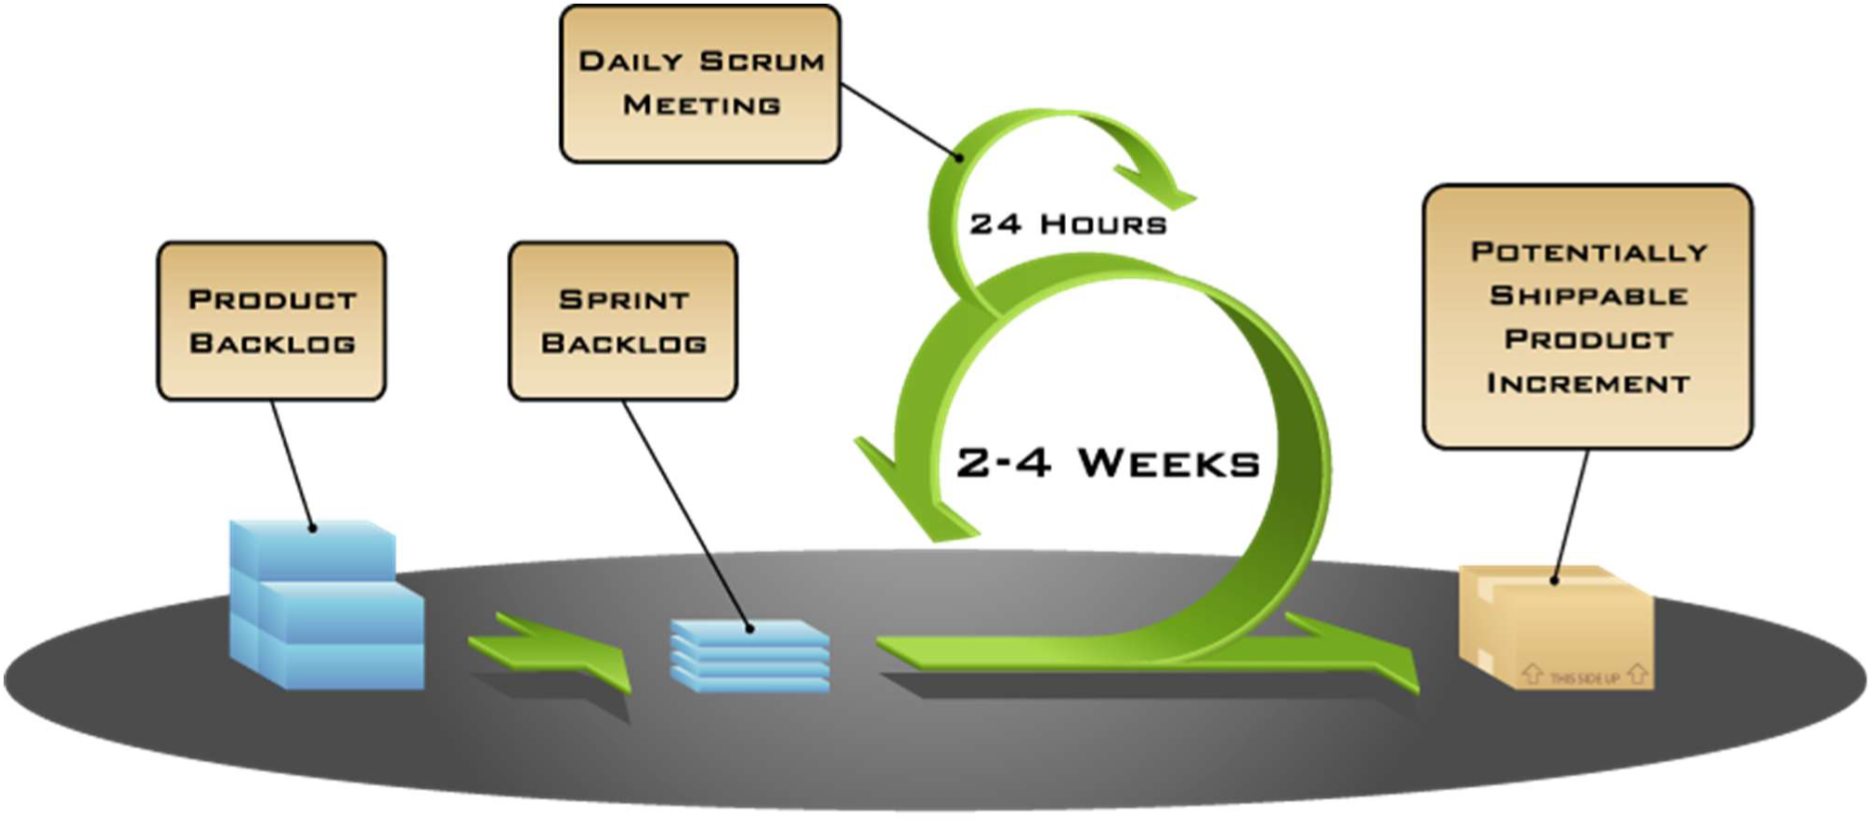
\includegraphics[width=400px]{img/HowScrumWorks.png}
	\captionof{figure}{How Scrum works}
	\label{fig:How Scrum works}
\end{Figure}

\subsection{Product Backlog}
\begin{itemize}
	\item Anforderungen
	\item Liste aller auszuführenden Arbeiten im Projekt
	\item Priorisiert
	\item Repriorisiert am Anfang jedes Sprints
\end{itemize}

\subsection{Sprints}
\begin{itemize}
	\item Scrum-Projekte machen in Form von Sprints fortschritte
	\item Typische Dauer 2-4 Wochen
	\item Länge der Sprints bleibt gleichbleibend
	\item konstante Dauer ist ein besserer Rhythmus
	\item jeder Sprint startet sofort nach den vorangangenden
	\item Während Sprints designed, codiert und getestet
	\item Der Umfang eines Sprints (Scope) wird immer neu verhandelt
\end{itemize}
\textbf{WICHTIG!} Während eines Sprints gibt es keine Änderungen $\rightarrow$ Die Länge der Sprints hängt davon ab, wie lange verhindert werden kann, dass Änderungen ins Projekt einfliessen



\section{Bestandteile von Scrum}
\begin{Figure}
\centering
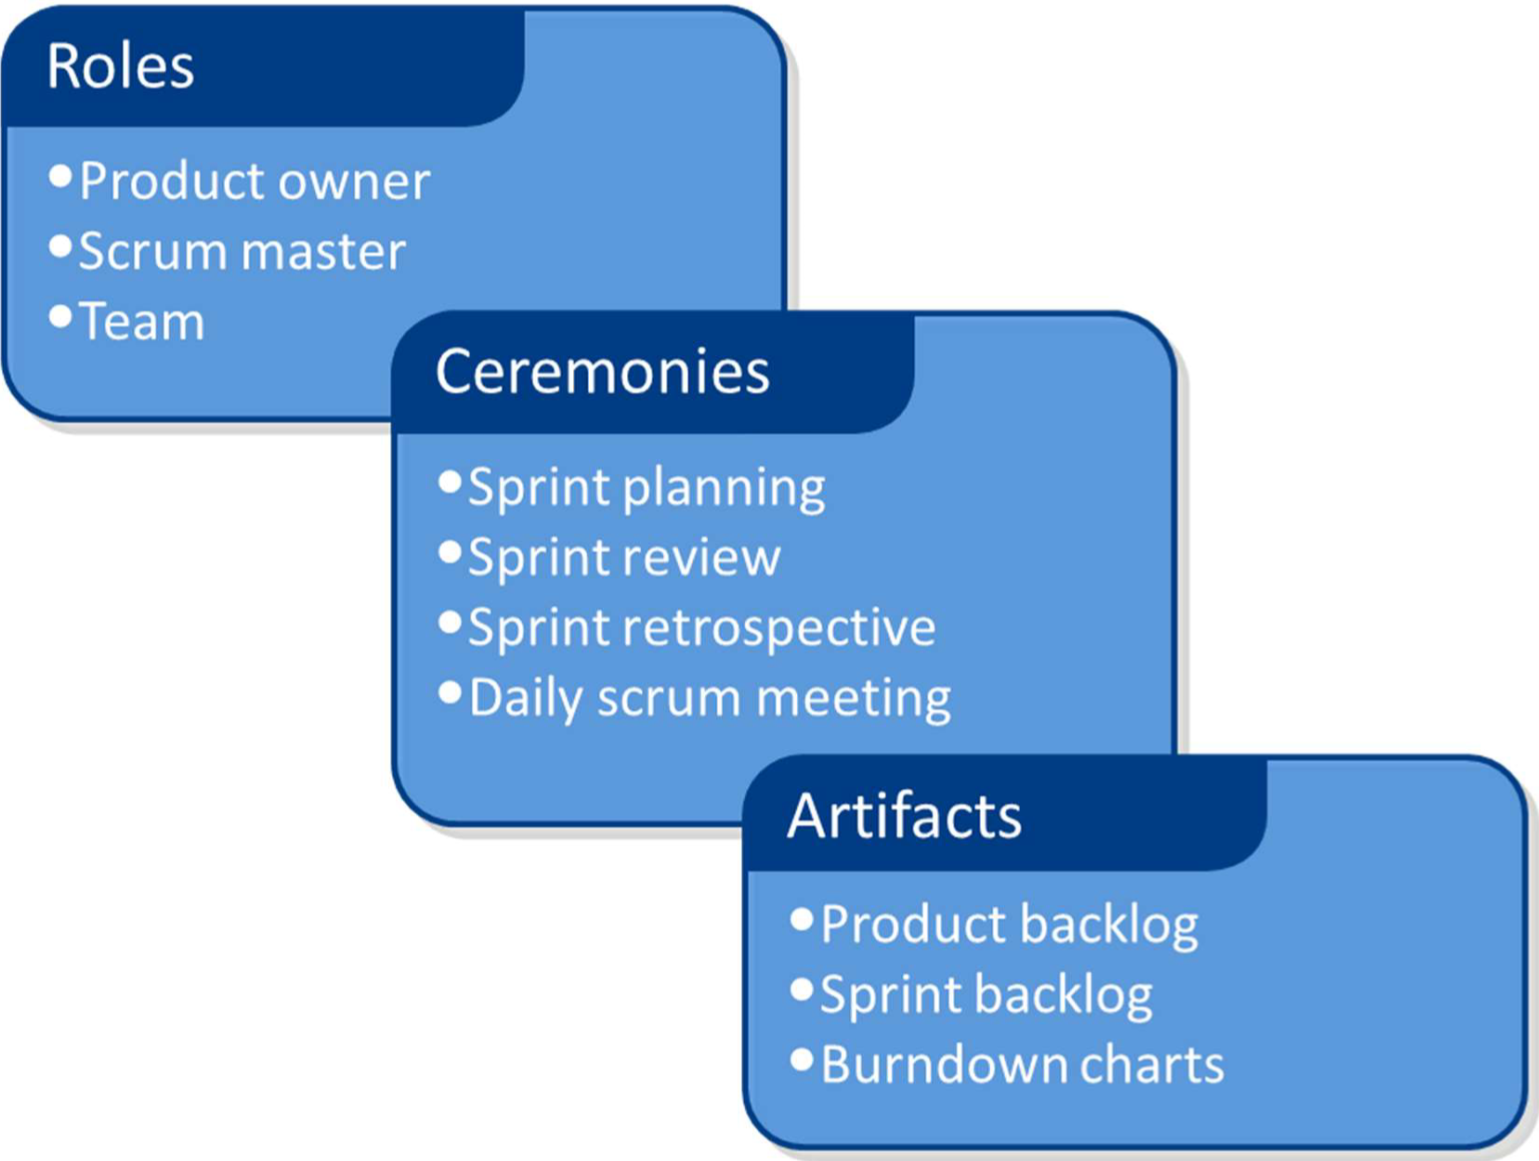
\includegraphics[width=400px]{img/BestandteileScrum.png}
	\captionof{figure}{Die Bestandteile von Scrum}
	\label{fig:Die Bestandteile von Scrum}
\end{Figure}

\subsection{Roles / Rollen}
Die drei Rollen in Scrum sind \textit{Product Owner, Scrum Master und Team}

\subsubsection{Product Owner}
\begin{itemize}
	\item Definiert Funktionen (Features) des Produktes
	\item Entscheidet über das Datum und den Inhalt eines Releases
	\item Ist verantwortlich für die Profitabilität (ROI) des Produktes
	\item Priorisiert Funktionen aufgrund ihres Marktwertes
	\item Passt Funktionen und Prioritäten, wenn nötig für jeden Sprint an
	\item akzeptiert Arbeitsresultate bzw. weist sie zurück
\end{itemize}

\subsubsection{Scrum Master}
\begin{itemize}
	\item Verantwortlich für die Durchsetzung der Scrum-Werte und Praktiken
	\item Entfernt Hindernisse
	\item Sorgt dafür, dass das Team vollständig arbeitsfähig und produktiv ist
	\item ermöglicht enge Zusammenarbeit zwischen allen Beteiligten
	\item Schirmt das Team gegen äussere Einflüsse ab
\end{itemize}

\subsubsection{Team}
\begin{itemize}
	\item Typischerweise 5-9 Personen
	\item Cross-functional $\rightarrow$ Programmierer, Tester, Designer etc.
	\item sollten zu 100\% im Team sein
	\item Selbst-organisierend
	\item Zusammensetzung sollte nur zwischen den Sprints ändern
\end{itemize}

\subsection{Ceremonies / Zeremonien}
Zur Zeremonie gehören folgende Elemente \textit{Sprint planning, Sprint Review, Sprint Retrospective, Daily Scrum Meeting}

\subsubsection{Sprint Planning}
\begin{itemize}
	\item Team wählt Items, die sie innerhalb eines Sprints umsetzen könne, aus dem Backlog aus
	\item Ein Sprint Backlog wird definiert
	\item Identifikation und Schätzung der Tasks (1-16h)
	\item Gemeinsam, nicht alleine durch den Scrum Master
	\item High-Level Design überlegen
\end{itemize}
Teil des Sprint Planning ist das \textit{Sprint Planning Meeting}
\begin{Figure}
\centering
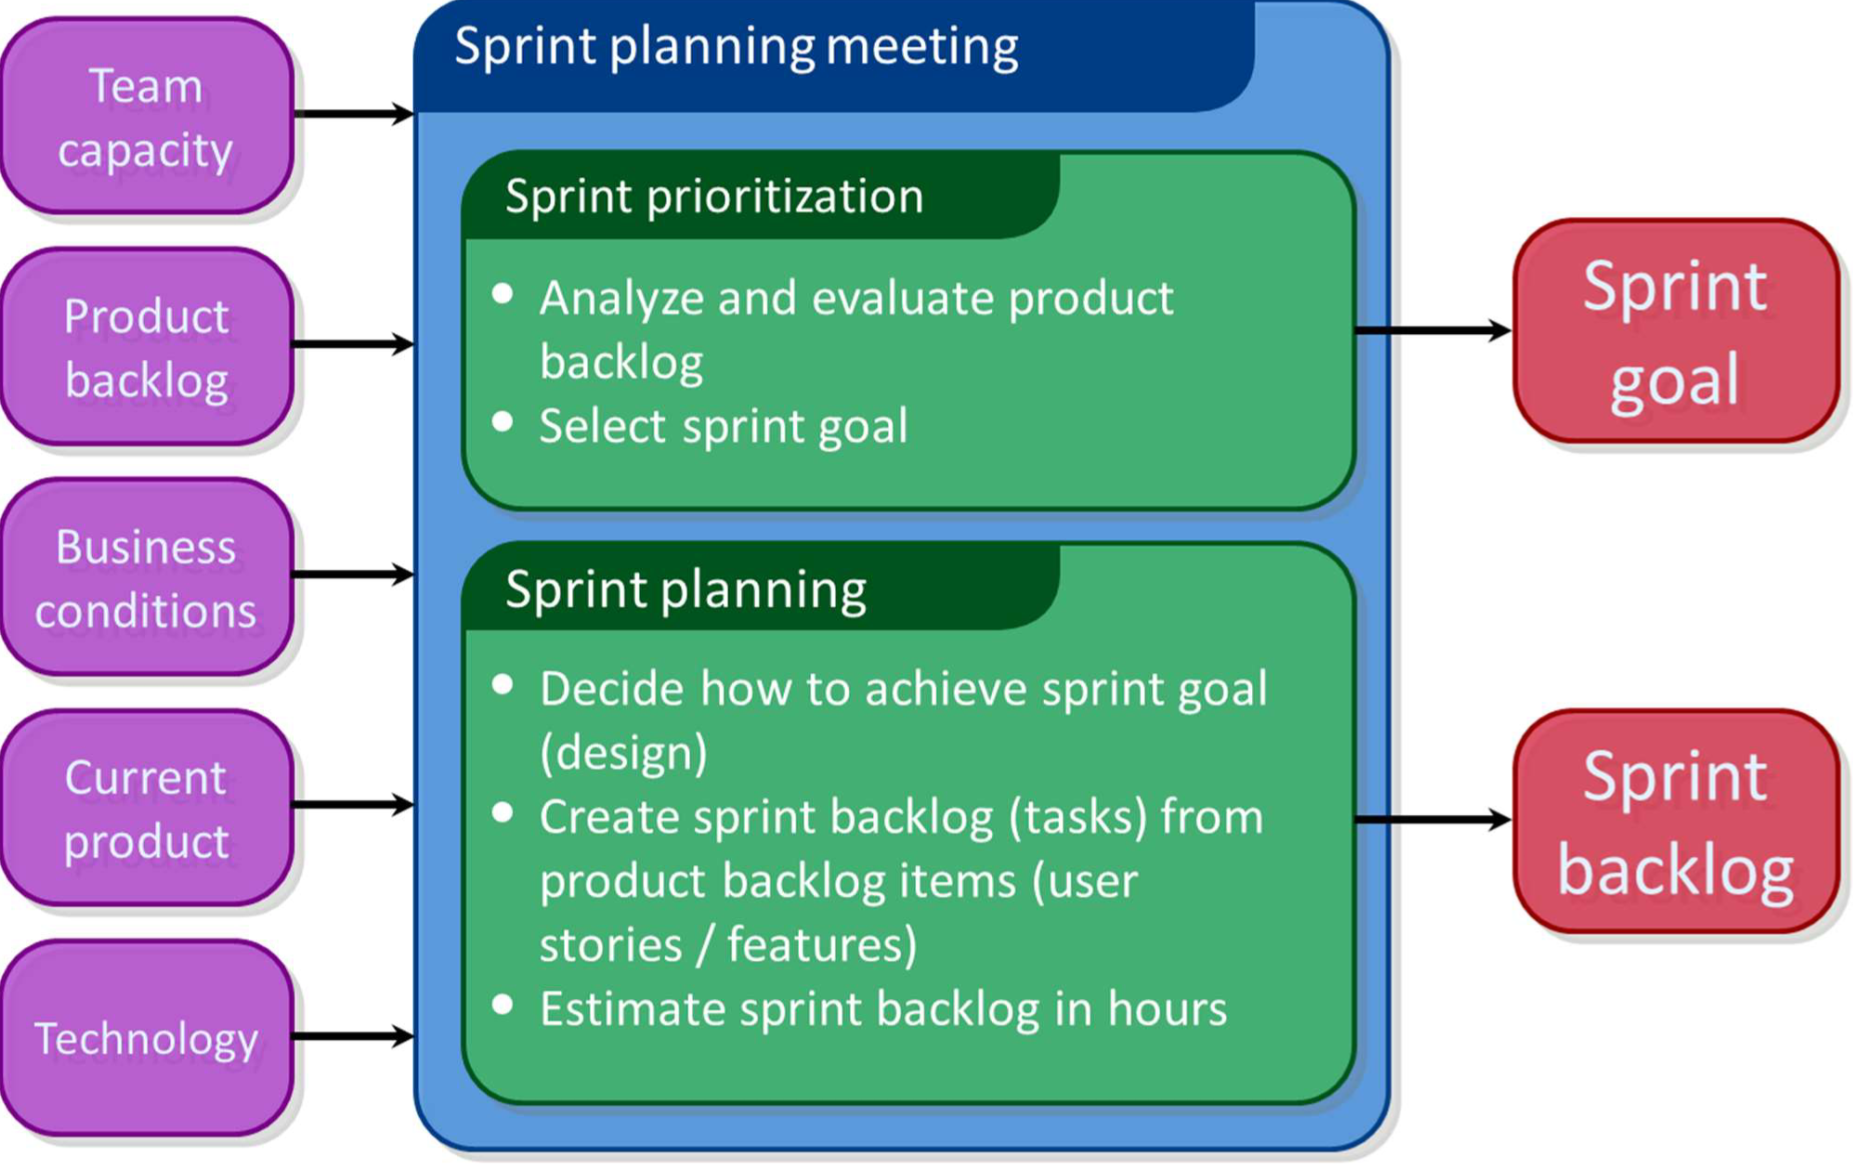
\includegraphics[width=400px]{img/SprintPlanningMeeting.png}
	\captionof{figure}{Sprint Planning Meeting}
	\label{fig:Sprint Planning Meeting}
\end{Figure}

Mit dem \textit{Sprint Goal} folgt ein kurzes Statement zur Zielformulierung
\subsubsection{Sprint Review}
\begin{itemize}
	\item Team präsentiert die Resultate des Sprints
	\item Als Demo (neue Funktionen / Architektur) $\rightarrow$ informell, 2h Vorbereitungszeit
	\item keine Folien
	\item alle nehmen teil
	\item alle einladen
	\item Feedback steht im Zentrum
	\item 4h für einen 4 Wochen Sprint
\end{itemize}

\textbf{Mechanismen eines Sprint Reviews}
\begin{itemize}
	\item { Product Owner Shares
			\begin{itemize}
				\item Was wurde erledigt
				\item Was wurde nicht erledigt
				\item Status des Produkt Backlogs
				\item ungefähre Release Abschätzung
			\end{itemize}
	}
	\item { Development Team Shares
			\begin{itemize}
				\item Fortschritt der Software
				\item Was wurde im Sprint realisiert
				\item Wie Probleme angegangen wurde und wie diese den Fortschritt beinflusst haben
			\end{itemize}
	}
	\item { Alle
			\begin{itemize}
				\item gibt und nimmt Feedback
			\end{itemize}
	}
\end{itemize}
\begin{Figure}
\centering
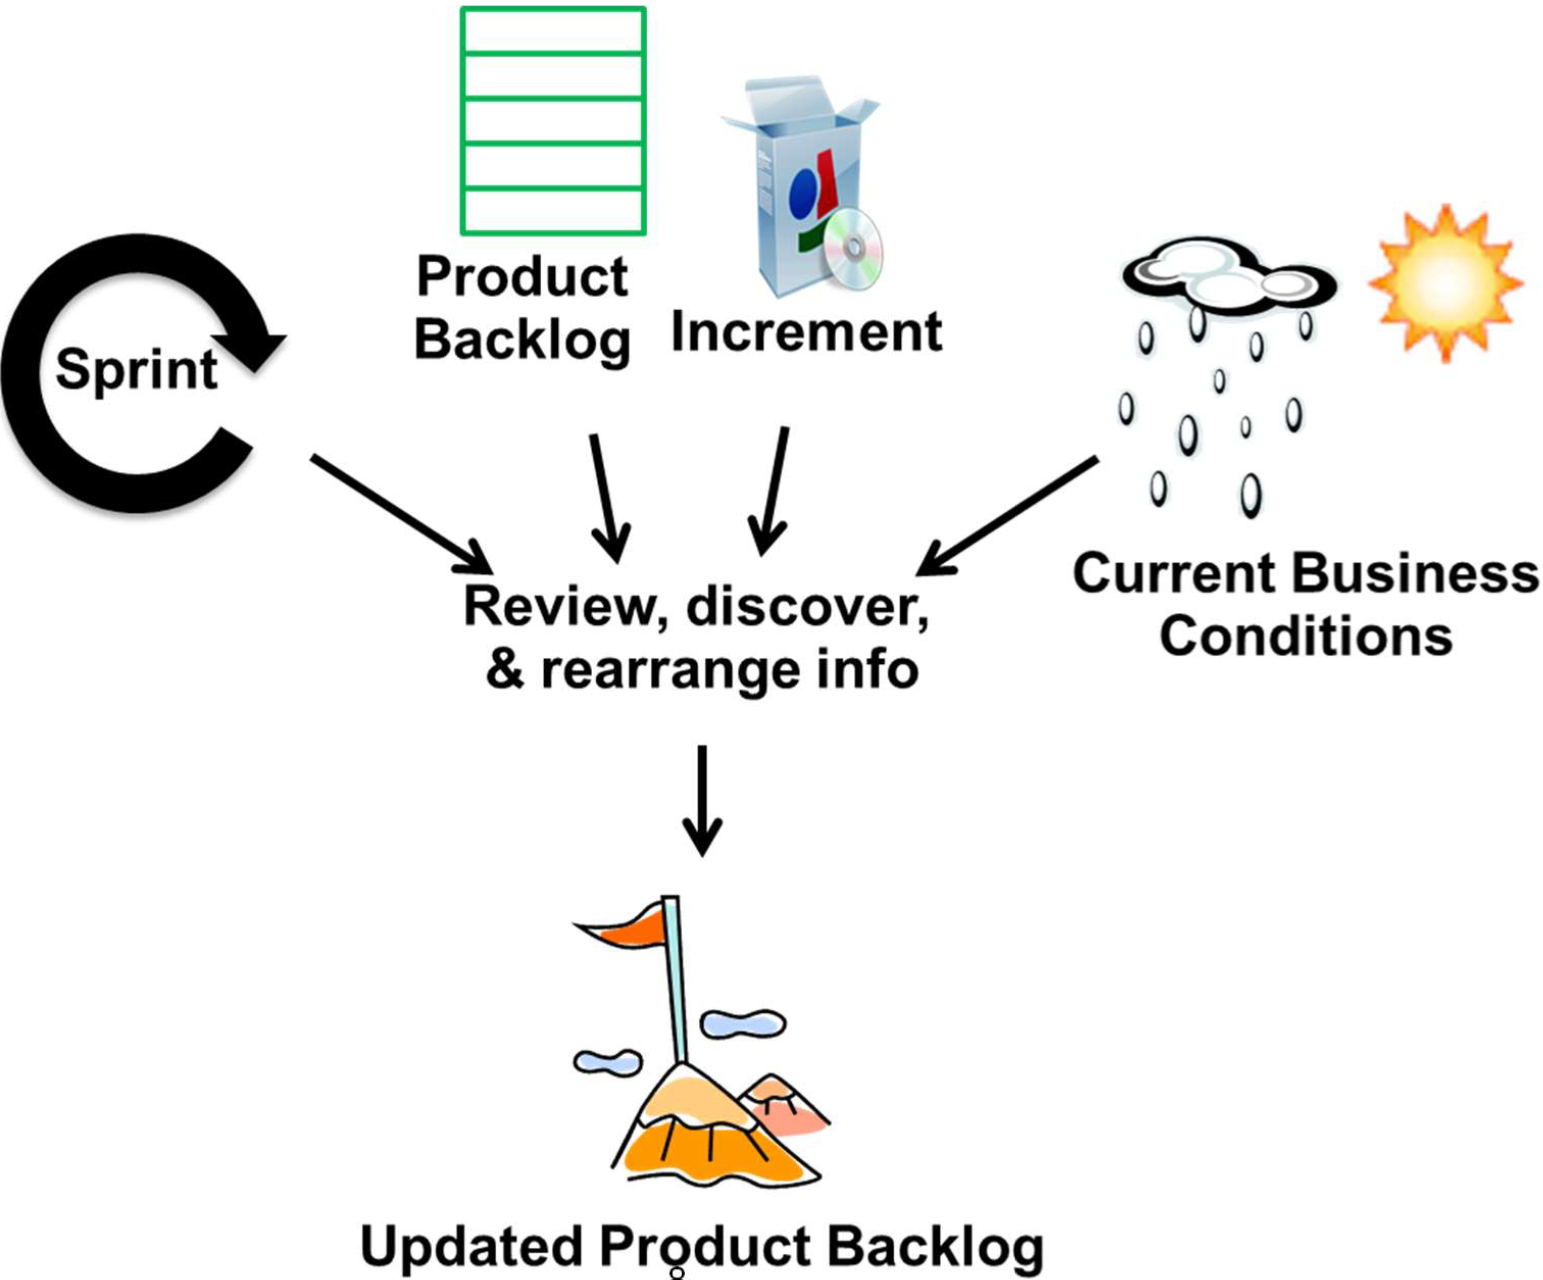
\includegraphics[width=400px]{img/InformationsflussReviewMeeting.png}
	\captionof{figure}{Informationsfluss eines Review Meetings}
	\label{fig:Informationsfluss eines Review Meetings}
\end{Figure}

\textbf{Checklisten}
\begin{itemize}
	\item {Ziel des Sprints
		\begin{itemize}
			\item Situation (Produkt Vision, Roadmap, Release Plan, Story map)
			\item Ziel
			\item Kapazität (Story Points, Aufwand)
			\item Review Kandidaten (Zielunterstützung, User Story OK, Alle verstehen Zielsetzung)
		\end{itemize}
	}
	\item {Backlog
		\begin{itemize}
			\item Für jede User Story (Priorität, Verständnis, Umsetzung, wie liefern, Aufwand, alles berücksichtigt?)
			\item Backlog Verifikation (Konflikte, Definition of Done, Fehlende Backlog Einträge, Risiken, Commitment, Tooling)
		\end{itemize}
	}
	\item Schluss (Nächste Schritte und Issues)
\end{itemize}

\subsubsection{Sprint Retrospective}
\begin{itemize}
	\item Periodische Prüfung was läuft und was nicht $\rightarrow$ Diskussion über Scrum Prozess, Verhalten der Teams, Tools, Erweiterung von 'Definition of Done'
	\item typischerweise 15-30 Minuten
	\item wird nach jedem Sprint durchgeführt
	\item Alle nehmen teil inkl. Kunden
	\item findet nach jedem Sprint Review statt
	\item {typische Fragestellungen
		\begin{itemize}
			\item Was funktionierte gut?
			\item Was können wir verbessern?
			\item Zu was commiten wir uns für den nächsten Sprint?
		\end{itemize}
	}
\end{itemize}

\textbf{Das Leitmotiv der Retrospektive}: \textit{Wir gehen davon aus, dass alle Beteiligten den bestmöglichen Einsatz im gegebenen Rahmen (Wissen, Ressourcen, Fähigkeiten) geleistet haben unabhängig davon, was im Rahmen einer Retrospektive entdeckt worden ist}

\subsubsection{Daily Scrum}
\begin{itemize}
	\item Parameter (täglich, 15 Minuten, Stand-Up)
	\item keine Problemlösungen
	\item alle Beteiligten sind eingeladen
	\item Nur die Team-Mitglieder, Scrum-Master oder Product Owner dürfen sprechen
	\item sollte unnötige Meetings vermeiden
\end{itemize}

Jeder Antwortet auf die folgenden Fragen:
\begin{enumerate}
	\item 'Was hast du gestern gemacht?'
	\item 'Was willst du heute tun?'
	\item 'Ist alles auf gutem Weg?'
\end{enumerate}

\subsection{Artifacts / Artefakten}
Die Artefakten beinhalten folgende Elemente \textit{Product Backlog, Sprint Backlog, Sprint Burndown Charts}

\subsubsection{Sprint Backlog}
\begin{itemize}
	\item Individuel wählen die Arbeit selbst aus $\rightarrow$ eine Zuweisung von Arbeit findet niemals statt
	\item Die Schätzung des noch verbleibenden Aufwandes erfolgt täglich
	\item Jedes Team-Mitglied kann den Sprint Backlog anpassen (CRUD)
	\item Die Arbeit des Sprints entsteht
	\item Falls die Arbeit unklar ist sollte ein entsprechend grösseres Backlog Item für die spätere Klärung geschaffen werden
\end{itemize}

\subsubsection{Sprint Burndown Chart}
\begin{itemize}
	\item Der Sprint Burndown Chart indiziert, wie gut ein Sprint vorwärts kommt
	\item Der Scrum Master sorgt dafür, dass das Team auf Warnsignale reagiert
\end{itemize}
\begin{Figure}
\centering
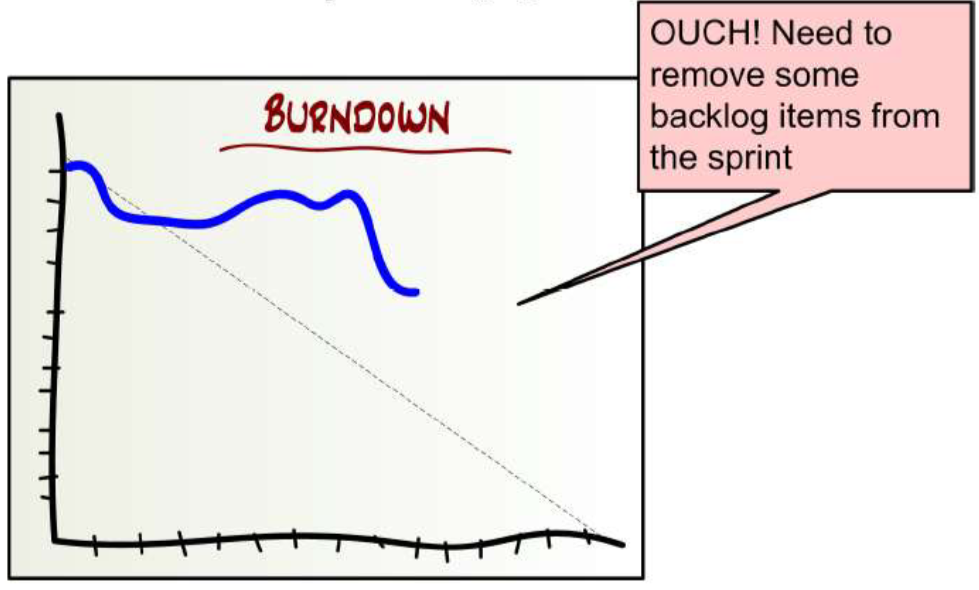
\includegraphics[width=400px]{img/Warnsignal1.png}
	\captionof{figure}{Burndown Chart Warnsignal 1}
	\label{fig:Burndown Chart Warnsignal 1}
\end{Figure}

\begin{Figure}
\centering
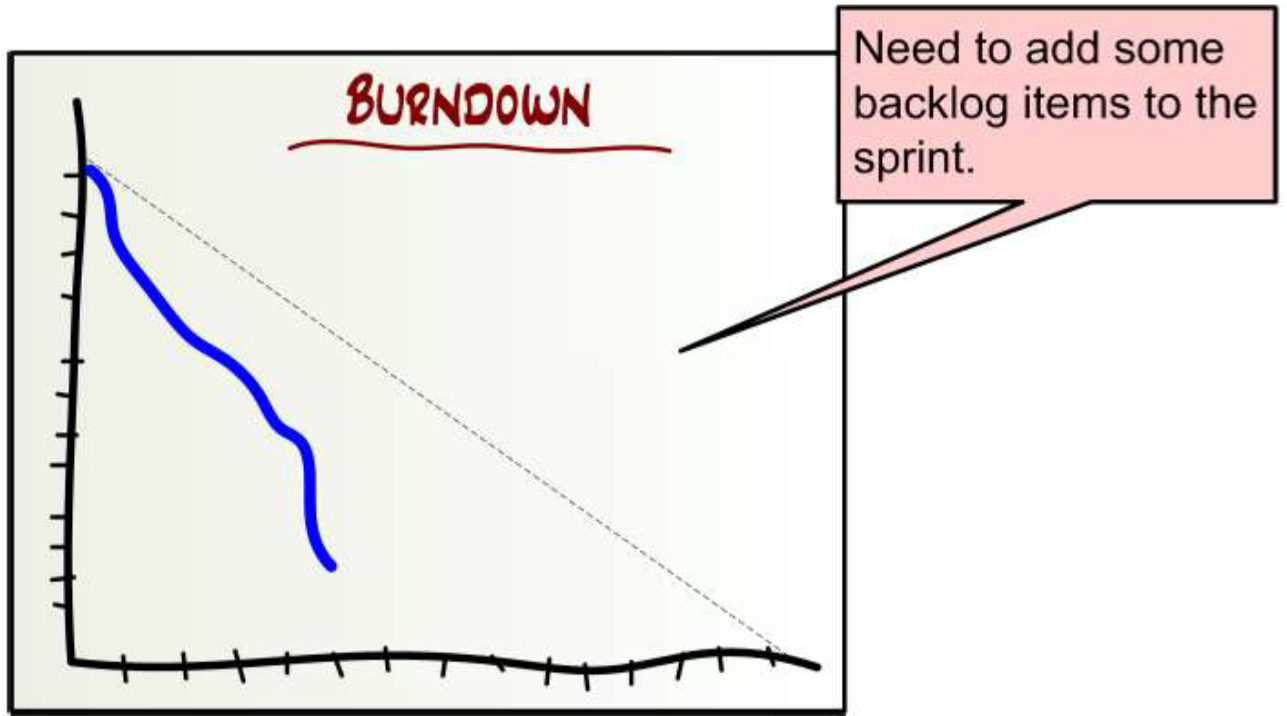
\includegraphics[width=400px]{img/Warnsignal2.png}
	\captionof{figure}{Burndown Chart Warnsignal 2}
	\label{fig:Burndown Chart Warnsignal 2}
\end{Figure}

\section{Skalierbarkeit}
\textit{Was ist Skalierbar}
\begin{itemize}
	\item Typische Grösse eines Teams: 7 +/- 2 Personen
	\item Die Skalierbarkeit wird durch Team of Teams erreicht
\end{itemize}

\section{Definition of Done (DoD)}
Ist eine Vollständigkeit im Sinne eines gegenseitig akzeptierten Übereinkommens aller Beteiligten, die Konform in Bezug auf die Governance-Vorgaben der Organisation ist. Wobei die Vollständigkeit in Bezug auf eine User Story und einen Sprint definiert ist.
\subsection{Konsequenzen bei fehlender DoD}
\begin{itemize}
	\item technische Schulden
	\item Nichterledigte Arbeit türmt sich
	\item Illusion in Bezug auf Projektfortschritt (Velocity)
	\item Unvorhersehbares Lieferdatum
	\item Team 'over-commitment' in Bezug auf die Arbeit, die während eines Sprints erledigt werden kann
	\item Der Product Owner liefert 'überraschende' Ergebnisse während dem Sprint Review
\end{itemize}

\subsection{Wer, Wie, Wann?}
\textbf{Wer} $\rightarrow$ Das Team inkl. Product Owner
\textbf{Wie} $\rightarrow$ Schriftlich im Einverständnis des gesamten Teams unter Einbezug des Product Owner und Kunden
\textbf{Wann} $\rightarrow$ Vor jedem Sprint und immer wieder adaptiert

\subsection{DoD für eine User Story}
\begin{enumerate}
	\item User Story ist definiert
	\item Akzeptanzkriterien sind definiert
	\item Schätzung durch das Team liegt vor
	\item Das Team hat die Artefakten des Nutzererlebnis akzeptiert
	\item Performance und andere nicht funktionale Eigenschaften sind definiert (falls notwendig)
	\item Die Abnahme-Person ist definiert
	\item Das Team hat eine klare Vorstellung, was gezeigt werden muss
\end{enumerate}

\subsection{DoD im ersten Sprint}
\begin{itemize}
	\item Wohin wird das erste Increment geliefert? und von wem?
	\item Welche Tests sollen diese erste Lieferung begleiten?
	\item Welche Dokumentation soll dieser ersten Lieferung beiliegen?
	\item Werden die heute bekannten Mängel immer noch präsent sein?
\end{itemize}

\section{Scrum beherrschen}

\subsection{Basics}

\subsubsection{Selbstorganisation}
Eine Struktur oder ein Pattern eines System, in welchem die Planung nicht durch eine zentrale Autorität oder ein anderes zentrales Element aufgezwungen wird $\rightarrow$ Die Fähigkeit von Teams sich selbst zu organisieren wird zum Vorteil einer Organisation verwendet.\\

\subsubsection{Selbstorganisation}
Damit dies funktioniert, braucht es ein gewisses Mass an Voraussetzung der Fähigkeiten
\begin{itemize}
	\item in Bezug auf die Domäne
	\item in Bezug auf die Rahmenbedingungen
	\item in Bezug auf die Entwicklung von Software
\end{itemize}

\subsubsection{Bedeutung}
Dies hat für die Teams folgende Bedeutung:
\begin{itemize}
	\item Wählen zu erledigende Arbeit selber aus
	\item Finden den besten Weg um Anforderungen zu erfüllen
	\item Suchen sich Hilfe zur Überwindung externer Hindernisse
	\item Wählen einen eigenen Scrum-Master
\end{itemize}

\subsubsection{Scrum-Diskussion}
Dabei gibt es zwei Seiten einer Scrum-Diskussion:
\begin{enumerate}
	\item { People Practices
		\begin{itemize}
			\item Planning
			\item Empiricism
			\item Collaboration
			\item Self-organziation
			\item Leadership
			\item Communication
			\item Transparency
		\end{itemize}
	}
	\item { Engineering Practices
		\begin{itemize}
			\item Design
			\item Coding
			\item Testing
			\item Automation
			\item Deploying
			\item User experience
			\item Emergent Architecture
		\end{itemize}
	}
\end{enumerate}

\subsection{Start im Unternehmen}
Agilität erfordert Umdenken $\rightarrow$ 'es war schon immer so' wird nicht mehr aktzeptiert, sondern es findet ein organisatorisches Umdenken statt

\textbf{Kotter's 8 Schritte}
\begin{enumerate}
	\item Dringlichkeit aufzeigen
	\item Führungskoalitation aufbauen
	\item Vision und Strategie entwickeln
	\item Die Vision kommunizieren
	\item Hindernisse aus dem Weg räumen
	\item Kurzfriste Erfolge sichtbar machen
	\item Veränderungen weiter antreiben
	\item Veränderungen in der Unternehmens-Kultur verankern
\end{enumerate}
$\Rightarrow$ Dies wird vom Product Owner und Scrum Master ausgeführt.


\subsection{Pflege von Scrum}
\textbf{tbd :-)}

\chapter{Architecture}

\section{Was bewirkt Architektur}
Die Qualität einer Software-Architektur hat einen Einfluss auf die ``allgemeinen Systemeigenschafte'' eines mittels der gewählten Architektur umgesetzten Systems. Diese Systemeigenschaften werden wiederum in zwei Gruppen aufgeteilt:\\
\begin{enumerate}
	\item Eigenschaften, die zur Laufzeit eines Systems gemessen werden können
	\item Eigenschaften, die nur indirekt gemessen werden können
\end{enumerate}

\begin{Figure}
\centering
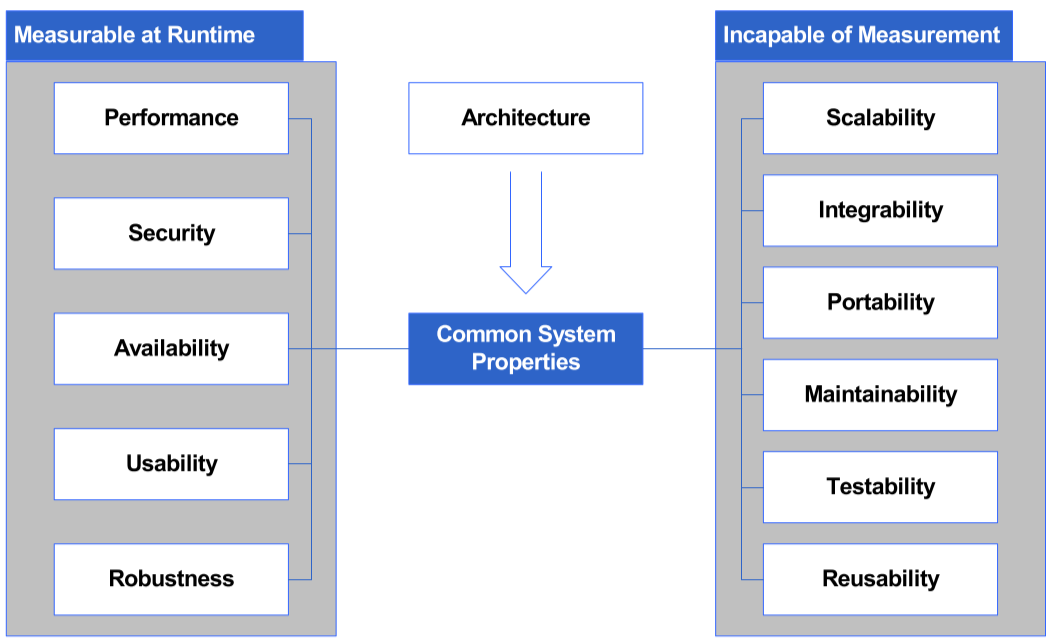
\includegraphics[width=400px]{img/WirkungArchitektur.png}
	\captionof{figure}{Was bewirkt Architektur}
	\label{fig:Was bewirkt Architektur}
\end{Figure}

\subsection{zur Laufzeit messbare Eigenschaften}
\begin{itemize}
	\item \textbf{Performance (Reaktionszeit / Durchsatz)} $\rightarrow$ geforderte Antwortszeiten werden garantiert. Systemantwortzeit hat wesentlichen Einfluss auf die Produktivität der Arbeit.
	\item \textbf{Security (Sicherheit)} $\rightarrow$ Schutz vor unautorisiertem Zugriff und mutwilliger Zerstörung
	\item \textbf{Availability (Verfügbarkeit)} $\rightarrow$ Muss zur Verfügung stehen und Mindestanforderungen erfüllen
	\item \textbf{Usability (Verwendbarkeit)} $\rightarrow$ Muss für den vorgesehen Zweck eingesetzt werden können
	\item \textbf{Robustness (Stabilität)} $\rightarrow$ Muss stabil laufen und darf unter Last nicht seinen Dienst teilweise oder ganz einstellen
\end{itemize}

\subsection{Nicht zur Laufzeit messbare Eigenschaften}
\begin{itemize}
	\item \textbf{Scalability (Skalierbarkeit)} $\rightarrow$ Muss ausgebaut werden können
	\item \textbf{Integrability (Integrierbarkeit)} $\rightarrow$ Nahtlose Integration mit existierende Umgebung
	\item  \textbf{Portability (Portablilität)} $\rightarrow$ Muss verschiedene Plattformen unterstützen
	\item \textbf{Maintainability (Wartbarkeit)} $\rightarrow$ Muss definierte Wartungsschnittstellen aufweisen und klar und übersichtlich strukturiert sein
	\item \textbf{Testability (Testbarkeit)} $\rightarrow$ Muss als Ganzes und in seinen einzelnen Komponenten testbar sein. Das Testen muss vom System selbst durch Hilfsmittel (Logs, Traces) unterstützt werden)
	\item \textbf{Reusability (Wiederverwendbarkeit)} $\rightarrow$ Systemteile müssen sich für andere Systeme wiederverwenden lassen
\end{itemize}

\section{Defintion: Was ist Architektur}
Allgemein ausgedrückt ist Architektur die Kunst oder Wissenschaft des planvollen Entwurfs der menschlichen Umwelt.

\subsection{diverse Definitionen}
\textbf{Zachmann}: \textit{Eine Architektur ist eine Menge von Gestaltungsgrundsätzen oder beschreibenden Darstellung, die relevant sind zur Beschreibung eines Objektes, sodass es gemäss Anforderungen produziert werden kann und während eines Lebenszyklus unterhalten werden kann}\\
\\
\textbf{IEEE}: \textit{Architektur: Die organisierte Struktur eines Systems oder einer Komponente}\\
\\
\textbf{ANSI / IEEE}: \textit{Architektur ist definiert als die grundlegende Organisation eines Systems, eingebettet in seinen Kopmonenenten, deren Beziehungen untereinander und der Umgebung, und als die Prinzipien die das Design und die Evolution des Systems beherrschen}\\
\\
\textbf{Booch, Rumbaugh und Jacobson (UML)}: \textit{Eine Architektur ist eine Menge von signifikanten Entscheidungen über die Organisation eines Software-Systems, der Auswahl der einzelnen Strukturelemente und deren Schnittstellen sowie deren Verhalten.}

\subsection{Die Formel der Architektur}
Die Architektur beinhalten gemäss Perry und Wolf folgende Elemente: Elements, Form, Rationale.
\begin{Figure}
\centering
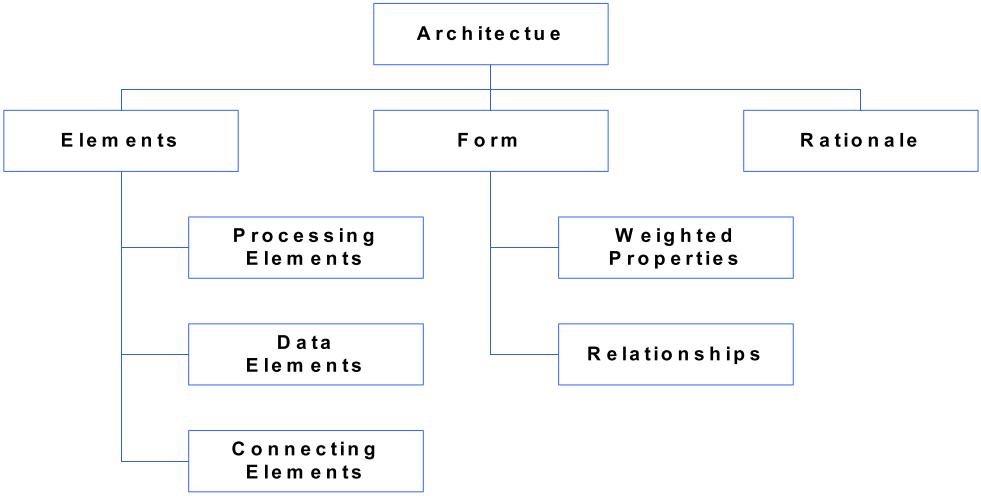
\includegraphics[width=400px]{img/ArchitekturFormel.png}
	\captionof{figure}{Architektur-Formel}
	\label{fig:Architektur-Formel}
\end{Figure}

\textbf{Elements}: Die Elemente einer Architektur sind entweder \textit{Processing Elements}, \textit{Data Elements} oder \textit{Connecting Elements}:
\begin{itemize}
	\item \textbf{Processing Elements} $\rightarrow$ Diese Elemente führen Transformationen auf Data Elements aus
	\item \textbf{Data Elements} $\rightarrow$ Sämtliche Daten eines Systems werden als Data Elements einer Architektur beschrieben
	\item \textbf{Connection Elements} $\rightarrow$ Connection Elements können entweder Processing Elements oder Data Elements oder beides sein. Bspw. Procedure Calls, Shared Data oder Messages
\end{itemize}

\textbf{Form}: Die Form einer Architektur wird beschrieben durch \textit{Weighted Properties} und \textit{Relationsships}:
\begin{itemize}
	\item \textbf{Weighted Properties} $\rightarrow$ Die Gewichtung von Eigenschaften eines Eleements erlaubt es einer Architektur zwischen zentralen und dekorativen Eigenschaften zu unterscheiden. Die Properties sind in einer Architektur ein Mittel zur Definition der Rahmenbedingungen eines Elements der Architektur. Sie definiere die minimalen Anfroderung, die ein Element erfüllen muss.
	\item  \textbf{Relationships} $\rightarrow$ werden zur Definition der Platzierung eines Elementes in einem bestimmten KOntext von Elementen verwendet
\end{itemize}

\textbf{Rationale}: Sie ist Ausdruck der Abbildung der Systemanforderungen, die von funktionalen hin zu allgemeinen Systemanforderungen reicht.

\section{Architektur und Prinzipien des Software Designs}

\subsection{Prinzipien}
\begin{itemize}
	\item \textbf{Modularity (Modularität)} $\rightarrow$ Komponenten eines Designs sollten aus leicht austauschbaren, verständlichen und in sich geschlossenen Teilen bestehen (bspw. ACL, DB Access, Validator, Rule Engine)
	\item  \textbf{Portability (Portabilität)} $\rightarrow$ Portabilität ist dann gegeben, wenn eine Software (oder Teile davon) so gestaltet werden, dass sie auch in anderen Umgebungen lauffähig sind
	\item \textbf{Changeability (Formbarkeit)} $\rightarrow$ Je formbarer ein System, desto leichter sind diese Änderungen durchzuführen
	\item \textbf{Conceptual Integrity} $\rightarrow$ Diejenigen Teile eines Systems, die ähnliche Funktionen beinhalten, sollten auch ähnlich gestalten werden (Industrie-Standards, Referenzarchitektur)
	\item \textbf{Intellectual Control} $\rightarrow$ Ein Software Design sollte von den Zuständigen hinsichtlich Form, Inhalt und Komplexität detailliert verstanden werden (Schnittstelle, Umfang)
	\item \textbf{Buildability} Ein Software Design muss ein Zielsystem so spezifizieren, dass es von einem gegebenen Team in einer gegeben Zeit realisiert werden kann (Know-how, Technologie)
\end{itemize}

\subsection{Kopplung und Kohäsion}
$\Rightarrow$ Je höher die Kohäsion individueller Module desto geringer die Kopplung

\subsubsection{Varianten der Kopplung:}
\begin{itemize}
	\item \textbf{Data Coupling} $\rightarrow$ Daten werden zwischen Modulen eines Systems ausgetauscht
	\item \textbf{Stamp Coupling} $\rightarrow$ Datenstrukturen werden zwischen Modulen eines Systems ausgetauscht
	\item \textbf{Control Coupling} $\rightarrow$ Der Austausch der Daten zwischen Modulen steuert den Kontrollfluss
	\item \textbf{Common Coupling} $\rightarrow$ Verschiedene Module greifen auf dieselben Daten
	\item \textbf{Content Coupling} $\rightarrow$ Ein Modul verändert die internen Daten eines anderen Moduls.
\end{itemize}
\subsubsection{Varianten der Kohäsion:}
\begin{itemize}
	\item \textbf{Coincidential Coehsion} $\rightarrow$ Die Gruppierung der Funktionalität eines Moduls erfolgt durch Zufall
	\item \textbf{Logical Coehsion} $\rightarrow$ Funktionalität in einem Modul zusammengefasst, beziehen sich jedoch nicht aufeinander
	\item \textbf{Temporal Cohesion} $\rightarrow$ Zeitpunkt der Verwendung bestimmt die Gruppierung der Funktionen
	\item \textbf{Procedural Coehsion} $\rightarrow$ Die Aufrufabfolge der Funktionen bestimmt die Gruppierung
	\item \textbf{Communcation Coehsion} $\rightarrow$ Gruppierung der Funktionalität wird durch den gemeinsamen I/O bestimmt
	\item \textbf{Sequential Coehsion} $\rightarrow$ Die Abfolge der Datenbearbeitung bestimmt die Gruppierung. Funktionen, deren Outpunt gleichzeitig zum Input für andere Funktionen wird, werden in einem Modul zusammengefasst
	\item \textbf{Functional Coehsion} $\rightarrow$ Diese Gruppierung hat zum Ziel, dass ein Modul Logik und Daten lokal halten kann (\textit{Information Hiding})
\end{itemize}

\subsubsection{Wirkung von Kopplung und Kohäsion}
\begin{itemize}
	\item \textbf{Design-Unabhängigkeit} $\rightarrow$ Jedes Modul kann unabhängig von anderen Modulen entworfen werden und spätere Änderungen finden nur und ausschliesslich in einem Modul statt. \textit{Vorraussetzung:} konstant gehaltene Definition der Schnittstellen, sowie einfrieren der Modulspezifikation
	\item \textbf{schmale Schnittstellen} $\rightarrow$ Anzahl der Meldungen zwischen Modulen ist klein
	\item  \textbf{wenig Schnittstellenverkehr} $\rightarrow$ Häufigkeit des Informationsaustausches zwischen vers. Modulen ist gering
	\item \textbf{Einheit} $\rightarrow$ Ähnliche Problemstellungen und Anforderungen werden ähnlich umgesetzt und entsprechend klassiert und gruppiert
	\item \textbf{Kapselung} $\rightarrow$ Abhängige Module werden zu grösseren Einheiten zusammengefasst
\end{itemize}

\subsection{Design for Change}
\begin{itemize}
	\item \textbf{Domain-Specific Changes} $\rightarrow$ Änderungen, die in ähnlichen System bereits realisiert werden mussten. Erfahrungsgemäss ändern sich bestimmte Systeme aufgrund ihres Kontextes (absehbar aufgrund betrieblicher / fachlicher Anforderungen wie bspw. Workflow, User und Rollen)
	\item \textbf{Analytical Changes} $\rightarrow$ Pflichtenhefte sind oft ungenau, Änderungen am System sind voraussehbar, da in vielen Fällen nicht jedes Detail der Spezifikation verifiziert werden kann.
	\item \textbf{Downsizing Changes} $\rightarrow$ Diese Änderungen erfolgen aufgrund von Budgetbeschränkungen und führen dazu, dass bestimmte Funktionalität weggelassen werden muss
\end{itemize}

\section{Schwierigkeiten und Vorteile der Architektur}

\subsection{No Silver Bullet}
4 Faktoren, die den Bau von Software so schwierig gestalten:
\begin{enumerate}
	\item \textbf{Komplexität} $\rightarrow$ Software ist im Verhältnis zu seiner grösse sehr komplex. Wird durch Abstraktion ein vereinfachtes Modell eines komplexen Phänomens erzeugt, so ist für das Modell wesentlich, dass in ihm die wichtigsten Eigenschaften des Phänomens abgebildet werden können. Die anderen Eigenschaften können weggelassen werden. Dies ist jedoch bei Software nicht der Fall. Es können keine Eigenschaften weggelassen werden, um die Komplexität in einfachere Modelle abzubilden.
	\item \textbf{Konformität} $\rightarrow$ Das Umfeld eines Systems (also Schnittstelle von einem System zum anderen) variieren in dem Masse, wie die Komplexität dieser Umsysteme variieren.
	\item \textbf{Formbarkeit} $\rightarrow$ Software unterliegt immerwährenden Veränderungen. Da Software so einfach geändert werden kann, werden auch sehr viele Änderungen durchgeführt.
	\item \textbf{Unsichtbarkeit} $\rightarrow$ Software ist unsichtbar und nicht direkt visualisierbar. Es existiert keine geometrische Repräsentation von Software. Die Visualisierung von Software verlangt verschiedene Sichten.
\end{enumerate}

\subsection{Vorteile guter Software Architektur}
\begin{itemize}
	\item Grundlage für die Kommunikation der an einem Softwareprojekt beteiligten Personen
	\item treibende Kraft des System-Designs fungieren
	\item Steckt den Rahmen für die Wiederverwendung einzelner Software-Artefakte ab
	\item 'Träger' von Qualitätscharakteristika und nichtfunktionaler Eigenschaften
	\item Invariante über mehrere Softwareprojekte mit minimal unterschiedlichen Systemanforderungen gelten und somit den Entwicklungsprozess für eine Serie ähnlicher Projekte vereinfachen
	\item Basis für eine umfassende Betrachtung einer Software und erlaubt die Analyse bestimmter Systemeigenschaften bereits zu einem sehr frühen Entwicklungszeitpunkt des Systems
\end{itemize}

\section{Standard-Stil-Pattern}
Das Vorgehen zur Abbildung von Anforderungen auf ein Zielsystem geht über drei Ebenen:
\begin{enumerate}
	\item \textbf{Architektur-Standards} $\rightarrow$ Auswahl und Anwendung des Architekturstandards
	\item \textbf{Architektur-Stil} $\rightarrow$ Auswahl und Anwendung der Kombination der verschiedenen Architektur-Stilelemente
	\item \textbf{Pattern} $\rightarrow$ Auswahl und Anwendung der passenden Entwurfsmuster
\end{enumerate}

\begin{Figure}
\centering
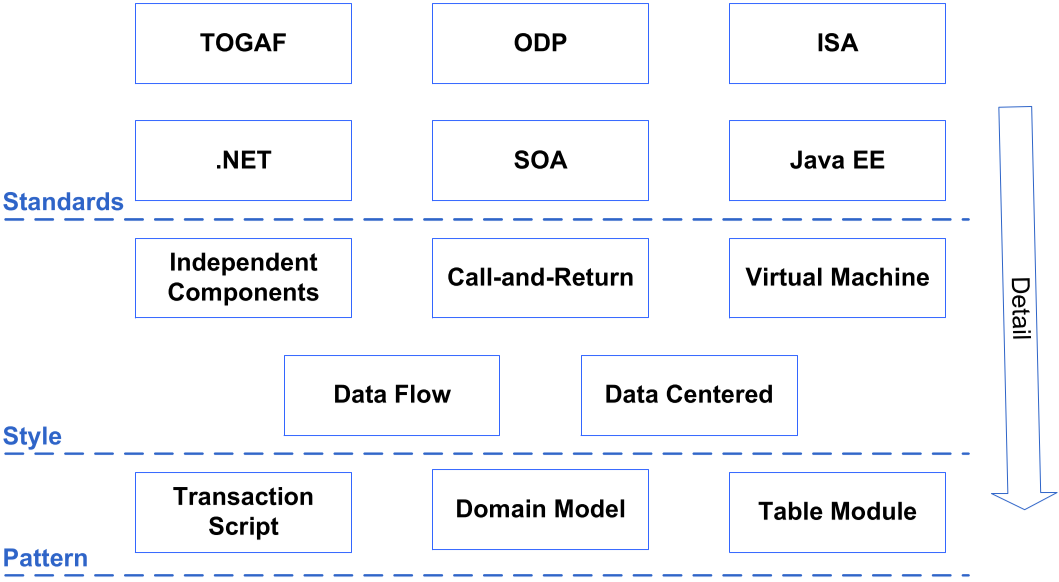
\includegraphics[width=400px]{img/StandardStilPattern.png}
	\captionof{figure}{Standard Stil Pattern}
	\label{fig:Standard Stil Pattern}
\end{Figure}

\section{Architektonischer Stil}

\subsection{Die vier Elemente eines Stils}
\begin{itemize}
	\item \textbf{Vocabulary} $\rightarrow$ Vokabular von Design-Elementen bestehend aus Komponenten (bspw. Server, Parser, DB) und Verbindungselementen (Remote Procedure Call, Data Streams oder Sockets).
	\item \textbf{Rules and Constraints} $\rightarrow$ Ein Architektur Stil unterliegt bestimmten Design-Regeln und Design-Einschränkungen, die definieren welche Elemente wie zusammengestellt werden können. Diese Regel vermeiden grundlegende Fehler in einem System Design
	\item \textbf{Semantics} $\rightarrow$ Bedeutung der verschiedenen Design-Elemente des Stils ist eindeutig. Semantische Regeln können zur Interpretation einer Komposition von Elementen herangezogen werden
	\item \textbf{Analytics} $\rightarrow$ Analytische Instrumente zur Prüfung des Vokabulars, Regeln und Einschränkungen eines bestimmte Architektur-Stils. Mit diesen Instrumenten können Kriterien wie die 'Schedulability' eines Real-Time Systems oder auch Deadlock Prevention eines Message-Passing Systems
\end{itemize}

\subsection{Übersicht Stile}

\subsubsection{Independent Components}
Unabhängig ablaufende Elemente, die über Nachrichten miteinander interagieren
\begin{Figure}
\centering
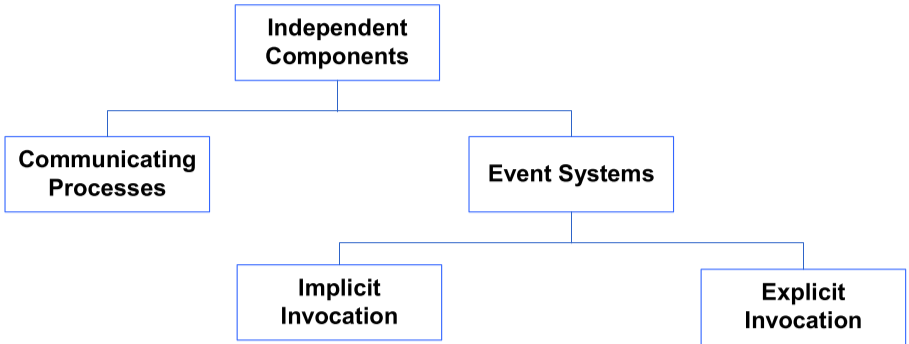
\includegraphics[width=400px]{img/IndependentComponents.png}
	\captionof{figure}{Übersicht Independent Components}
	\label{fig:Übersicht Independent Components}
\end{Figure}

\textbf{Communicating Processes}\\
\textbf{Definition}: beliebige Anzahl miteinander kommunizierender Elemente. Die Synchronisation erfolgt ausschliesslich über die Kommunikationskanäle zwischen den Elemente und kann sowohl synchron als auch asynchron erfolgen\\
\textit{Beispiel}: Springer Problem $\rightarrow$ wird mittels Backtracking gelöst

\begin{Figure}
\centering
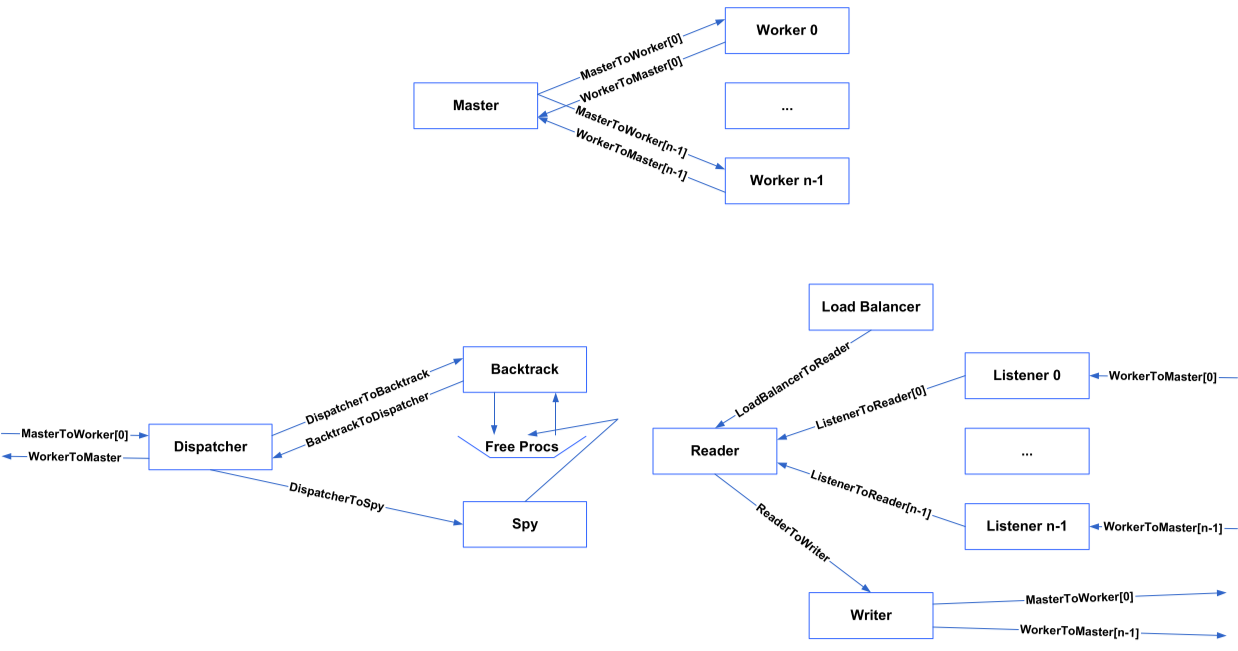
\includegraphics[width=400px]{img/CommunicatingProcessesBeispiel.png}
	\captionof{figure}{Beispiel eines communicating Processes}
	\label{fig:Beispiel eines communicating Processes}
\end{Figure}

\textbf{Event-Systems}\\
Dieser Ereignisgesteuerte Architektur Stil definiert Architekturen, deren Prozesse über Events miteinander kommunizieren.
\begin{itemize}
	\item \textbf{Implicit Invocation} $\rightarrow$ Sämtliche Events werden an einen so genannten Event Space gesendet, der dann die Verteilung der Events an die betroffenen Prozesse.
	\item \textbf{Explicit Invocataino} $\rightarrow$ Die Events werden direkt zwischen den einzelnen Prozessen ausgetauscht
\end{itemize}
\textit{Beispiel} MVC / Message Broker

\begin{Figure}
\centering
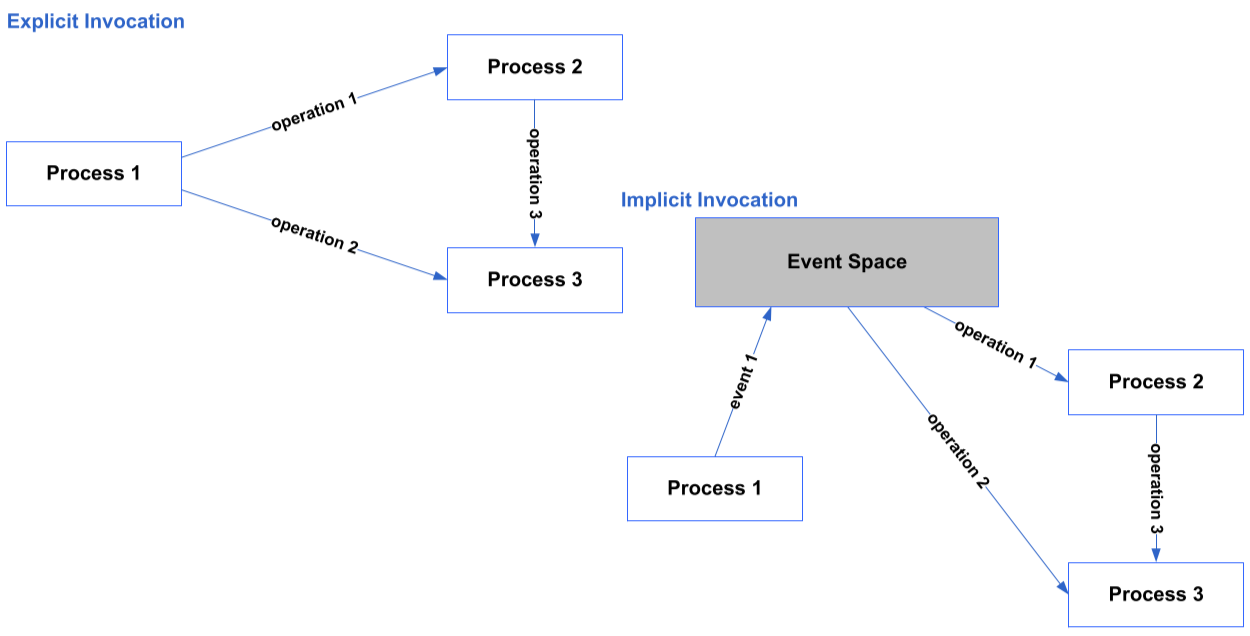
\includegraphics[width=400px]{img/EventSystems.png}
	\captionof{figure}{Event Systems}
	\label{fig:Event Systems}
\end{Figure}

\subsubsection{Call-and-Return}
Definiert durch einen fixen Kommunikations-Mechanismus zwischen aufrufendem und aufgerufenen Element

\begin{Figure}
\centering
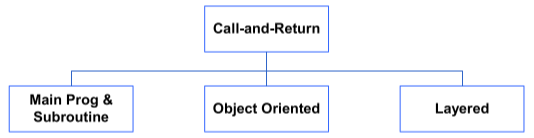
\includegraphics[width=400px]{img/CallAndReturn.png}
	\captionof{figure}{Übersicht Call and Return}
	\label{fig:Übersicht Call and Return}
\end{Figure}

\textbf{Main Program und Subroutine}
Repräsentiert das klassische Programmierparadigma der SASD (Structured Analysis - Structured Design) mit eindeutigem Kontrollfluss, der einen Baum bestehend aus Hauptprogrammen und unterprogrammen, wobei die Kontrolle dem gerade ausführenden Teil des Systems übertragen wird, durchläuft
\begin{Figure}
\centering
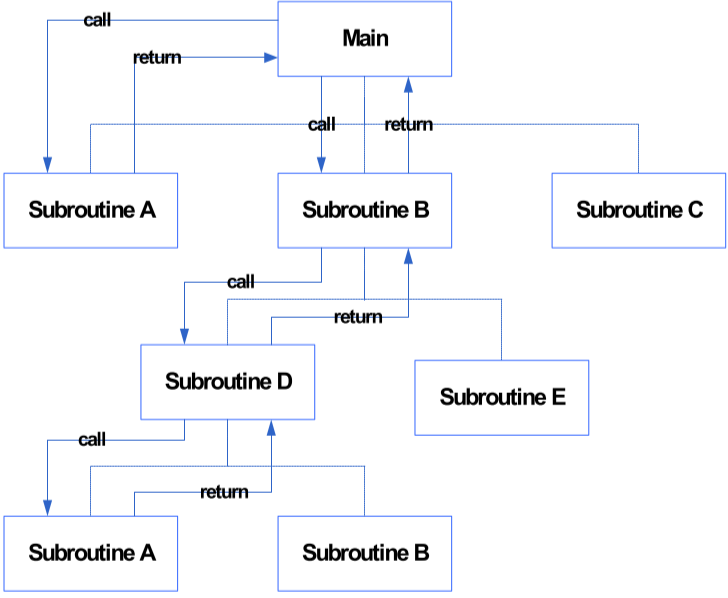
\includegraphics[width=400px]{img/MainProgramAndSubroutine.png}
	\captionof{figure}{Ablauf MainProgram and subroutine}
	\label{fig:Ablauf MainProgram and subroutine}
\end{Figure}

\textit{Beispiele}: Remote-Procedure-Call\\

\textbf{Layered Architecture}\\
Schichtenmodell, welches hierarchisch gegliedert ist. Teilt Aufgaben eines Gesamtsystems in Schichten auf. Das Spektrum der Elemente, die einer bestimmten Schicht zugeordnet werden können, wird eingeschränkt.
$\Rightarrow$ Stärken: Lokalität der Änderungen, Änderungen betreffen maximal die geänderte Schicht, sowie die untenliegende und die oben liegende Schicht. Falls an den Schnittstellen zwischen den Schichten nichts geändert wird, so ist sogar lediglich eine Schicht betroffen.\\
\textit{Beispiele}: Risk Management System $\rightarrow$ Bewertung und Isolation operativer Risiken durch Konsolidierung von Produktions- und Vertriebsdaten. Mit folgenden Layern (Presentation, Database, Backend)
\begin{Figure}
\centering
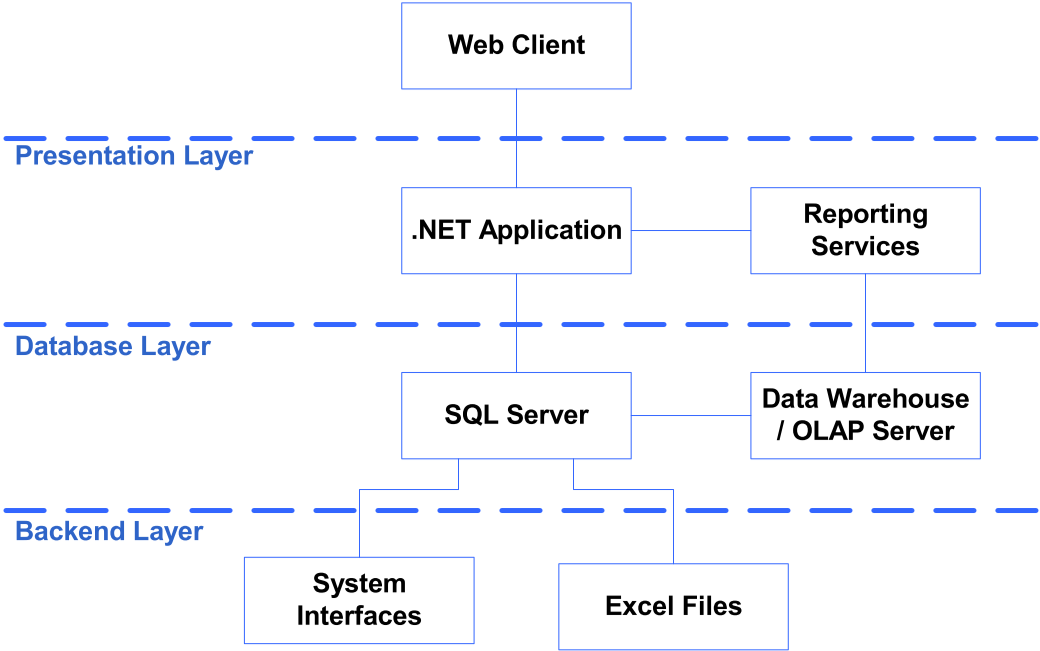
\includegraphics[width=400px]{img/LayeredArchitectureBeispiel.png}
	\captionof{figure}{Layered Architecture Beispiel}
	\label{fig:Layered Architecture Beispiel}
\end{Figure}

\subsubsection{Virtual Machine}
Erlaubt die Realisierung portabler und interpretierbarer Systeme
\begin{Figure}
\centering
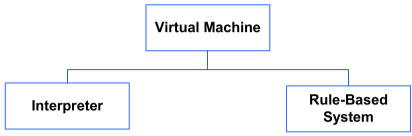
\includegraphics[width=400px]{img/VM.png}
	\captionof{figure}{Übersicht Virtual Machine}
	\label{fig:Übersicht Virtual Machine}
\end{Figure}

\textbf{Interpreter}\\
Eine abstrakte Maschine - also ein hypothetischer Computer mit den definierten Elementen für deren inneren Aufbau
\begin{Figure}
\centering
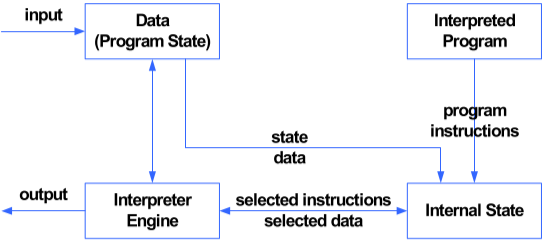
\includegraphics[width=400px]{img/Interpreter.png}
	\captionof{figure}{Übersicht Interpreter (VM)}
	\label{fig:Übersicht Interpreter (VM)}
\end{Figure}
\textit{Beispiel}: Java VM\\

\textbf{Rule Based System}
Generalisierung des Interpreter. Zentrale Eigenschaft ist die Trennung zwischen der Maschine an sich und den Regeln, die die Maschine beschreiben
\begin{Figure}
\centering
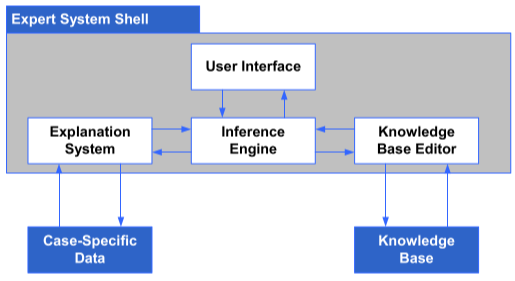
\includegraphics[width=400px]{img/RuleBasedSystem.png}
	\captionof{figure}{Rule Based System}
	\label{fig:Rule Based System}
\end{Figure}
\textit{Inference Engine}


\subsubsection{Data Flow}
System ist eine Abfolge von datenbezogenen Transformationen.\\
Der Data Flow Architekturstil umfasst Architekturen, die ein System als eine Abfolge von Transformationen auf sequentiellem Dateninput modellieren. Aktiviert und gesteuert wird das System durch vorliegende Daten. Diese Daten werden Schritt für Schritt durch das System geleitet, werden dabei verändert und schliesslich als ausgehende Daten bereitgestellt
\begin{Figure}
\centering
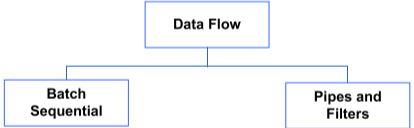
\includegraphics[width=400px]{img/DataFlow.png}
	\captionof{figure}{Data Flow}
	\label{fig:Data Flow}
\end{Figure}

\textbf{Batch Sequential}\\
Die Transformationen auf den Daten erfolgen durch voneinander unabhängige Elemente dieses Architekturstils. Dies bedeutet, dass die Daten als ganzes eingelesen werden, um dann transformiert und anschliessend wieder als Ganzes abgelegt zu werden.

\textbf{Pipes and Filters}\\
Die Transformationen auf den Daten erfolgen lokal (Filter) mittels Streaming (Pipes). Dies bedeutet, dass ein eingehender Data Stream laufend in einen ausgehenden Data Stream umgewandelt wird.

\subsubsection{Data Centered}
Zentrale Aufgabe ist Zugriff und Aktualisierung von Daten eines Repositories.\\
Der Datenzentrierte Architekturstil umfasst Architekturen, die Systeme beschreiben, deren zentrale Funktion der Zugriff auf Daten eines Repositoriers ist.
\begin{itemize}
	\item Passives Repository $\rightarrow$ Datenbank
	\item Aktives Repository $\rightarrow$ Blackboard
\end{itemize}
\textit{Bemerkungen}:\\
\begin{itemize}
	\item Ein Blackboard System sendet Nachrichten über geänderte Daten an interessierte Subscriber des Systems. Dieser Mechanismus ist sehr flexibel und skalierbar, da Blackboard Systeme die Datenhaltung von den angeschlossenen Clients trennen.
	\item Die Trennung zwischen passiven Datenzentrierten Sytemen und aktiven Datenzentrierten Systemen ist fliessend, da heute jede Datenbank mit Triggern sehr einfach in ein Blackboard System umgewandelt werden kann.
\end{itemize}

\chapter{OR Mapping mit JPA}

\section{Domain Model}
Das Domain Model ist klassischerweise ein Artefakt aus der Analyse und nicht ein Artefakte aus der Programmierung

\subsection{Das Pattern}
Anwendung von bewährten OO-Techniken für die Implementation der Geschäftslogik $\rightarrow$ Kapselung, Vererbung, Polymorphie, Design Patterns, ...\\
Dabei verspricht OO:
\begin{itemize}
	\item besser Skalierung bei zunehmender Komplexität
	\item bessere Erweiterbarkeit
	\item bessere Wartbarkeit
	\item weniger Redundanzen
\end{itemize}
\begin{Figure}
\centering
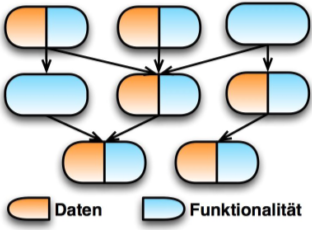
\includegraphics[width=200px]{img/JPAPattern.png}
	\captionof{figure}{Das Pattern vom Domain Model}
	\label{fig:Das Pattern vom Domain Model}
\end{Figure}

\subsection{Technologie}
\begin{itemize}
	\item Fokus auf reine objekt-orientierte Programmierung
	\item Kontrast zu Infrastruktur-lasten und OO-feindlichen Technologien wie EJB2 oder JDBC-Resultsets
\end{itemize}

\subsection{Architektur: Domain Layer}
\begin{itemize}
	\item Zentralisierung und Lokalisierung von Business Logik (DRY)
	\item Context independent $\rightarrow$ Persistence Ignorance
\end{itemize}

\begin{Figure}
\centering
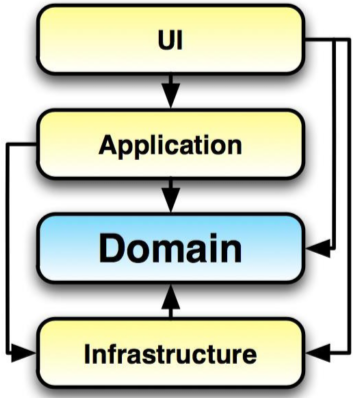
\includegraphics[width=200px]{img/JPADomainLayer.png}
	\captionof{figure}{Architektur des Domain Layer}
	\label{fig:Architektur des Domain Layer}
\end{Figure}

\subsubsection{typsiche Herausforderungen}
\begin{itemize}
	\item Peristence-Ignorance (Testbarkeit, Wiederverwendbarkeit, Freiheit im OO-Design) $\rightarrow$ ORM mit JPA bietet einen Lösungsansatz
	\item Zentralisierung der Validierungslogik (Validierung auf verschiedenen Ebenen bspw. UI, Business-Logik, DB) $\rightarrow$ Bean Validation bietet einen Lösungsansatz
\end{itemize}

\subsection{Klassen und Metadaten}
\begin{itemize}
	\item Klassen werden mit Metadaten angereichert
	\item Metadaten sind verantwortlich für einen speziellen (infrastruktur) concern
	\item Metadaten werden zur Laufzeit von einer Runtime konsumiert
	\item Kern-Logik bleibt entkoppelt von den Metadaten
	\item klassisch in XML
	\item Seit JDK5 als Annotations
\end{itemize}

\begin{Figure}
\centering
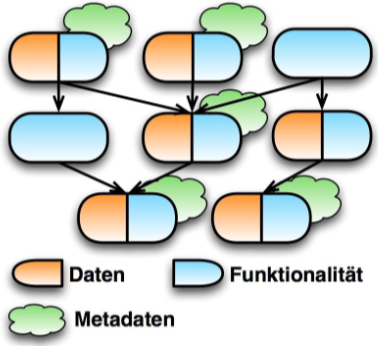
\includegraphics[width=300px]{img/JPAMetadaten.png}
	\captionof{figure}{Konzept von Klassen und Metadaten in JPA}
	\label{fig:Konzept von Klassen und Metadaten in JPA}
\end{Figure}

\subsection{Anwendbarkeit Domain Model Patterns}
\begin{itemize}
	\item Der Einsatz des Domain Model Patterns macht vor allem Sinn für die Umsetzung von komplexer, erweiterbarer und wartbarer Geschäftslogik
	\item Der Einsatz der Technologien JPA und BeanValidation kann auch ohne Umsetzung des Domain Model Patterns Sinn machen
\end{itemize}

\section{Einführung ORM und JPA}
Objektrelationales Mapping ist ein sehr umstrittens Thema

Die Ausgangslage des Domain Models wird im Kapitel oben beschrieben.


\subsection{Ausgangslage relationale Datenbanken}
\begin{itemize}
	\item Vorherrschende Technologie zum Speichern von Daten im Enterprise-Umfeld
	\item Grosse Investitionen
	\item Bewährte und ausgereifte Technologie
	\item Flexibilität
	\item Applikationsunabhängigkeit
	\item Daten leben länger als Applikationen
	\item Optimierte Konzepte zum Speichern von Daten
\end{itemize}

\subsubsection{der Konflikt}
De facto Standard-Konstellation für Enterprise-Applikationen: OO-Technologie für die Applikationsentwicklung. Relationale Datenbanken für die Persistenz der Daten. An dieser Ausgangslage wird sich mittelfristig kaum etwas ändern. Der OO-Ansatz und der relationale Ansatz weisen grundsätzliche Unterschiede auf. Aus diesen Unterschieden resultiert der sogenannte Object-Relational-Mismatch

\subsection{O/R-Mapping}
\subsubsection{Der O/R Mismatch}
\begin{itemize}
	\item In Enterprise Umfeldern ist O/R-Mismatch ein Fakt
	\item Folgt aus konzeptionellen Unterschieden der zugrundeliegenden Technologien
	\item verschiedene Möglichkeiten zur Überwindung $\rightarrow$ bspw. O/R-Mapping Frameworks
\end{itemize}

\textbf{Designziele}
\begin{itemize}
	\item {DB
		\begin{itemize}
			\item Speichern und Abfragen von Daten
			\item Speicherung unabhängig von konkreten Business-Problemen
		\end{itemize}
	}
	\item {OO
		\begin{itemize}
			\item Vereinigung von Zustand und Verhalten
			\item Kapselung, Modularisierung, Abstraktion
			\item Modellierung konkreter Business-Probleme
		\end{itemize}

	}
\end{itemize}

\textbf{Architekturansätze}
\begin{itemize}
	\item {DB
		\begin{itemize}
			\item Client / Server: verteiltes System
		\end{itemize}
	}
	\item {OO
		\begin{itemize}
			\item Objekte sind lokal und nicht verteilt
		\end{itemize}
	}
\end{itemize}

\textbf{Abfragen / Zugriff}
\begin{itemize}
	\item {DB
		\begin{itemize}
			\item Deklarative Abfragesprache
			\item Beziehungen zwischen Daten müssen nicht explizit definiert sein
		\end{itemize}
	}
	\item {OO
		\begin{itemize}
			\item Imperative Navigation entlang von Referenzen
			\item Beziehungen zwischen Objekten müssen explizit definiert sein
		\end{itemize}
	}
\end{itemize}

\subsubsection{Versprechen von O/R-Mapping}
\begin{itemize}
	\item {Applikation wird von DB entkoppelt
		\begin{itemize}
			\item Applikationsentwicklung muss kein SQL beherrschen
			\item relationale Modell der DB hat keinen Einfluss auf OO-Design
		\end{itemize}
	}
	\item {Automatische Persistenz
		\begin{itemize}
			\item automatisierte Abbildung der Objekte in die relationale Strukturen
			\item Entwickler muss sich nicht um die low-level Details des CLI (bspw. Connections) kümmern
		\end{itemize}
	}
	\item {Transparente Persistenz / Perstience Ignorance
		\begin{itemize}
			\item  Klassen des Domain-Models wissen nicht, dass sie persistiert und geladen werden können und haben keine Abhängigkeit zur Persistenz-Infrastruktur
		\end{itemize}
	}
	\item {Abstraktion
		\begin{itemize}
			\item eines der wichtigsten Werkzeuge
		\end{itemize}
	}
	\item {Separation of Concerns
		\begin{itemize}
			\item Bei der Applikationsentwicklung kann man sich ausschliesslich auf die Geschäftsprobleme konzentrieren
			\item Infrastruktur-Probleme können separat gelöst werden und beeinflussen das Design und die Implementation der Geschäftslogik nicht
		\end{itemize}
	}
\end{itemize}

\subsubsection{Versprechen von O/R-Mapping Frameworks}
\begin{itemize}
	\item Versprechen von O/R-Mapping
	\item Einsatz von bewährten Patterns und Konzepten
	\item Einsparung von viel Code
	\item Strukturierung / Layerung des Codes vorgegeben
\end{itemize}

$\Rightarrow$ \textbf{Pitfalls}\\
\begin{itemize}
	\item komplex und viel Funktionalität
	\item keine Rapid-Application-Development-Tools
	\item Einfluss auf Architektur und Design der gesamten Applikation
	\item zugrundeliegende Konzepte müssen verstanden sein
	\item gründliche Auseinandersetzung ist Voraussetzung für erfolgreichen Einsatz
\end{itemize}

\subsubsection{Konzeptionelle Probleme}
\begin{itemize}
	\item {\textbf{Location Transparency}
		\begin{itemize}
			\item Alle Daten immer verfügbar
			\item Für Applikation sollte es keinen Unterschied machen ob die Daten lokal oder auf entfernter DB gespeichert sind
			\item wie viele Daten sollen geladen werden (zuviele braucht Speicher und Bandbreite $\rightarrow$ Ladezeit, zu wenig muss konstant nachgeladen werden $\rightarrow$ Ladezeit
		\end{itemize}
	}
\end{itemize}

\subsubsection{Dynamisch generiertes SQL}
SQL ist nicht so performant wie handgeschriebenes, getuntes SQL. Dynamisch generiertes SQL muss auch nicht gewartet werden. Ausgereife Frameworks generieren gut optimiertes SQL. Dabei sind Stored Procedures nicht performanter als dynamisches SQL

\subsubsection{relationale Suche / Reports}
Nutzung von relationalen Konzepten, die keine Entsprechung in der OO-Welt haben.

\begin{Figure}
\centering
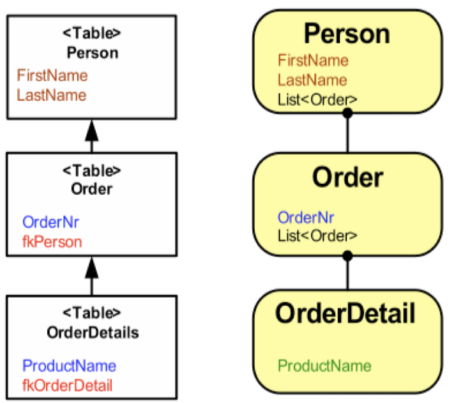
\includegraphics[width=400px]{img/JPARelationaleSuche.png}
	\captionof{figure}{Relationale / Reports}
	\label{fig:Relationale / Reports}
\end{Figure}

\textbf{Probleme}\\
\begin{itemize}
	\item {karthesisches Produkt
		\begin{itemize}
			\item in der DB sehr effizient
			\item in der OO-Welt keine Entsprechung
		\end{itemize}
	}
	\item {Struktur des Resultats der Anfrage exisiert nicht in der OO-Welt
		\begin{itemize}
			\item keinen Typ mit den Attributen
			\item relationale Welt erlaubt flexible (untypisierte) Sichten auf die Daten
			\item Resultat einer Anfrage kann völlig entkoppelt sein von der Struktur wie die Daten gespeichert werden
			\item die OO-Welt verlangt definierte, stark typisierte Strukturen
		\end{itemize}
	}
	\item Das Flachdrücken bzw. Denormalisieren muss in der OO-Welt manuell ausgeführt werden
	\item Alle beteiligten Objekte müssen geladen werden (Performance!)
\end{itemize}

\section{JPA Übersicht}

\subsection{Entity}
\begin{itemize}
	\item Entity ist persistierbar
	\item Zustand kann in Datenbank abgespeichert werden
	\item Entity hat eine Objektidentität und besitzt zusätzlich eine Datenbankidentität (Primary Key)
	\item Erstellung, Änderung und Löschen wird in einer Transaktion durchgeführt
\end{itemize}

\textbf{Entity Metadata}
\begin{itemize}
	\item Kennzeichnung mit Annotation ``@Entity'' oder Mapping mit XML
	\item Klasse als Basisklasse
	\item Klasse abstrakt oder konkret
	\item Serialisierbarkeit ist bzgl. Persistenz nicht erforderlich
	\item Schnittstelle für die Interaktion mit der Persistence Engine
\end{itemize}

\begin{Figure}
\centering
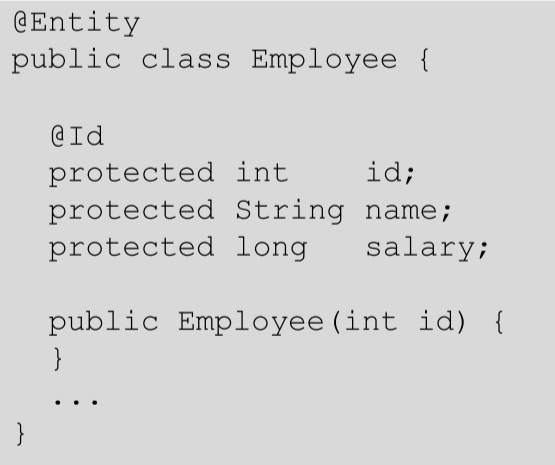
\includegraphics[width=400px]{img/EntityBsp.png}
	\captionof{figure}{Beispiel einer Entity}
	\label{fig:Beispiel einer Entity}
\end{Figure}

\begin{Figure}
\centering
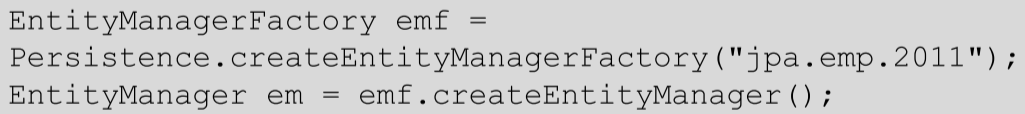
\includegraphics[width=400px]{img/emErstellen.png}
	\captionof{figure}{Entity Manager erstellen}
	\label{fig:Entity Manager erstellen}
\end{Figure}

\begin{Figure}
\centering
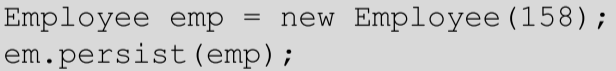
\includegraphics[width=400px]{img/EntityPersist.png}
	\captionof{figure}{Entity persistieren}
	\label{fig:Entity persistieren}
\end{Figure}

\begin{Figure}
\centering
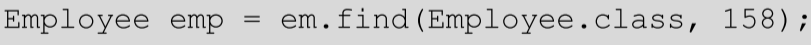
\includegraphics[width=400px]{img/EntitySearch.png}
	\captionof{figure}{Entity suchen}
	\label{fig:Entity suchen}
\end{Figure}

\begin{Figure}
\centering
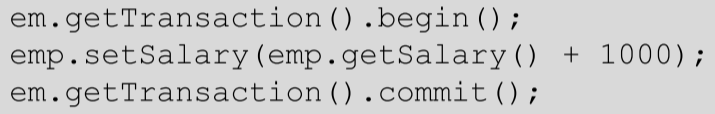
\includegraphics[width=400px]{img/EntityGetSet.png}
	\captionof{figure}{Entity verändern}
	\label{fig:Entity verändern}
\end{Figure}

\begin{Figure}
\centering
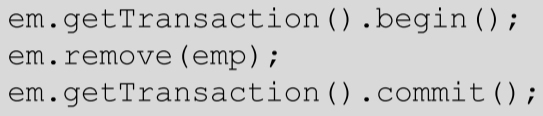
\includegraphics[width=400px]{img/EntityDelete.png}
	\captionof{figure}{Entity löschen}
	\label{fig:Entity löschen}
\end{Figure}

\begin{Figure}
\centering
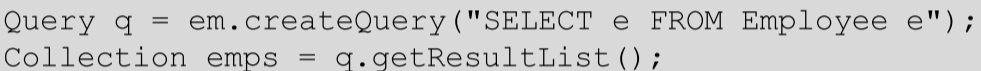
\includegraphics[width=400px]{img/EntityQuery.png}
	\captionof{figure}{Entity abfragen}
	\label{fig:Entity abfragen}
\end{Figure}

\begin{Figure}
\centering
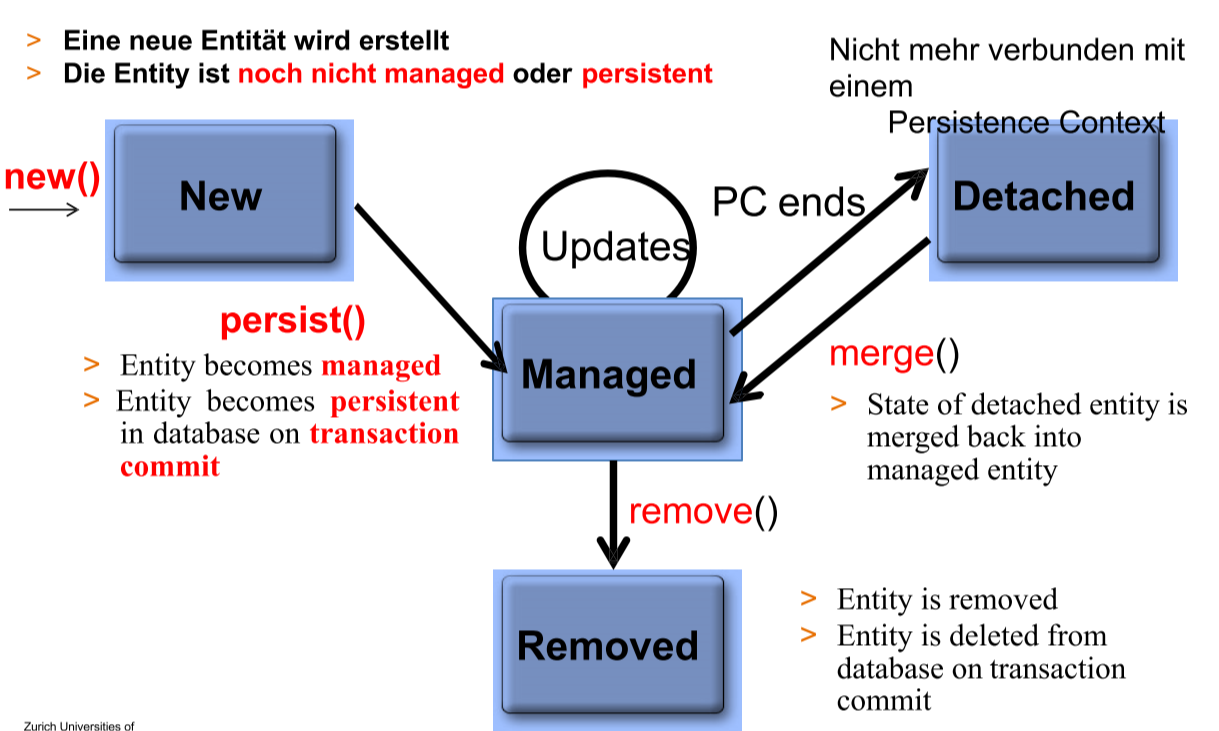
\includegraphics[width=400px]{img/EntityLifecycle.png}
	\captionof{figure}{Entity Lifecycle}
	\label{fig:Entity Lifecycle}
\end{Figure}


\subsection{Peristence}
\textbf{Perstistence Unit} Konfiguration für das Mapping der Entities mit einer relationalen Datenbank.\\
Ist eine logische Einheit von Entities

\subsection{Entity Mapping}
Mittels dem Mapping kann man die Verbindung zwischen Objekt und Datenbank herstellen. Dies wird mittels den unterschiedlichen Annotations erledigt.

\begin{Figure}
\centering
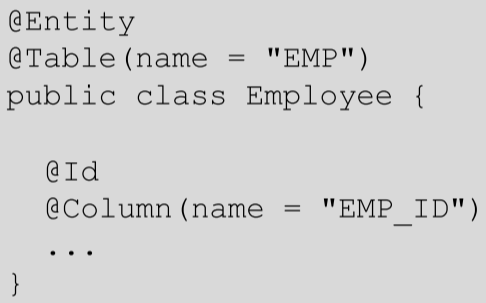
\includegraphics[width=400px]{img/MappingBsp.png}
	\captionof{figure}{Beispiel Mapping}
	\label{fig:Beispiel Mapping}
\end{Figure}

\textit{Was ist alles erlaubt?}
\begin{itemize}
	\item Alle primitiven Typen, String
	\item Alle Wrapperklassen und serialisierbaren Typen (bspw. Integer, BigDecimal, Date, Calendar)
	\item byte[], Byte[], char[], Character[]
	\item Enumerations
	\item bel. weitere Entity-Klassen
	\item Collections von Entities (Collection, List, Set, Map)
\end{itemize}

\textit{nicht erlaubt}
\begin{itemize}
	\item Alle Arten von Arrays ausser die obengenannten
	\item Collections von etwas anderem als Entities
\end{itemize}

\subsubsection{Lazy Field Loading}

\begin{Figure}
\centering
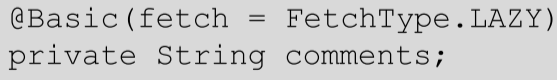
\includegraphics[width=400px]{img/LazyFieldLoading.png}
	\captionof{figure}{Lazy Field Loading}
	\label{fig:Lazy Field Loading}
\end{Figure}

\subsubsection{Large Objects}

\begin{Figure}
\centering
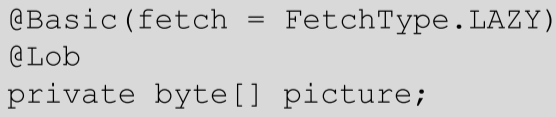
\includegraphics[width=400px]{img/LargeObjects.png}
	\captionof{figure}{Large Objects}
	\label{fig:Large Objects}
\end{Figure}

\subsubsection{Enumerations}
Enumerations können persistent sein. In der DB wird entweder der \textit{Ordinalwert} (Position) oder der \textit{Stringwert} (Name der Konstante) abgelegt

\begin{Figure}
\centering
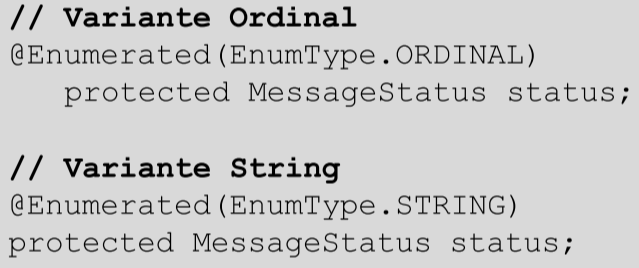
\includegraphics[width=400px]{img/MappingEnumerations.png}
	\captionof{figure}{Mapping Enumerations}
	\label{fig:Mapping Enumerations}
\end{Figure}

\subsubsection{Entity Identity - Primärschlüssel}
Jede Entity-Klasse muss einen mit ``@Id'' bezeichneten Primärschlüssel besitzen.\\
Eine Id kann von folgenden Typen sein
\begin{itemize}
	\item Primitive Java Typen
	\item Wrapper Klassen
	\item Array von primitiven Typen oder Wrapper Klassen
	\item java.lang.String
	\item java.math.BigInteger
	\item Zeittypen
	\item theoretisch auch Floating Point Typen, ist jedoch nicht zu empfehlen
\end{itemize}

\begin{Figure}
\centering
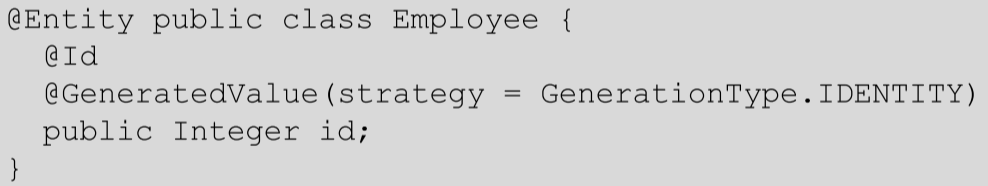
\includegraphics[width=400px]{img/EntityPrimaryKey.png}
	\captionof{figure}{Generierung von Primary Keys}
	\label{fig:Generierung von Primary Keys}
\end{Figure}

\subsection{Beziehungen}

\begin{Figure}
\centering
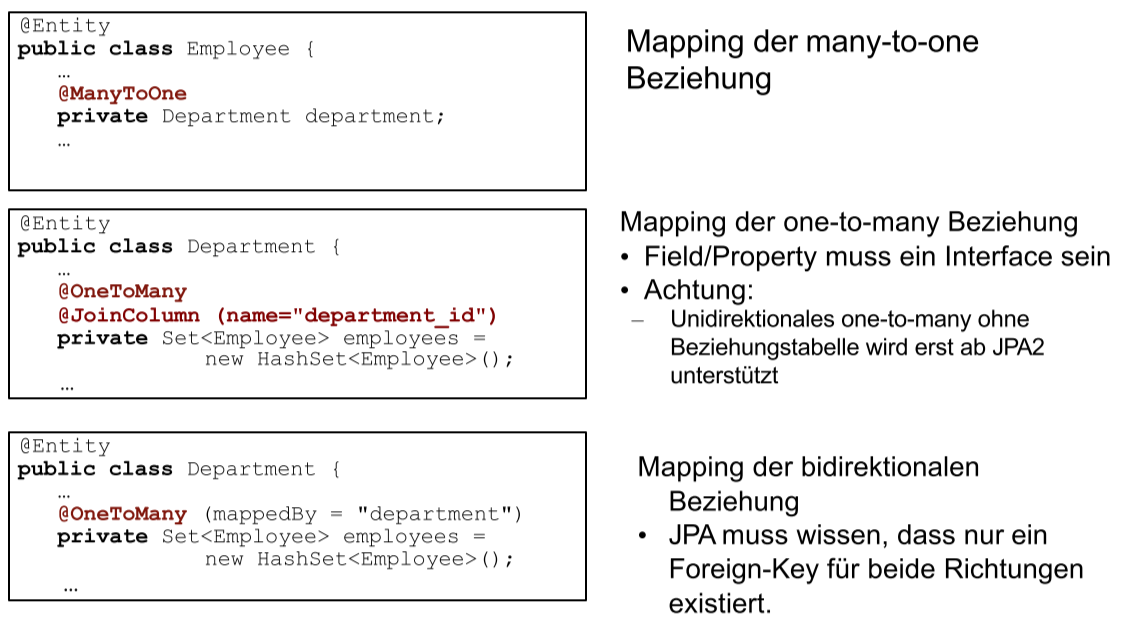
\includegraphics[width=400px]{img/ParentChildBeziehung.png}
	\captionof{figure}{Parent-Child Beziehung}
	\label{fig:Parent-Child Beziehung}
\end{Figure}

\textbf{TODO: Evtl. Woche10 ab Folie 70 ergänzen, falls notwendig}

\chapter{REST}
Funktionalität wird hinter einer Schnittstelle verbergt.

Akronym für \textbf{RE}presentational \textbf{S}tate \textbf{T}ransfer

\section{Einführung}
Grundlegende Designprinzipien
\begin{itemize}
\item REST-Server bietet Zugang zu Ressourcen
\item REST-Client manipuliert die Ressourcen mit HTTP-Methoden
\item Zustandslosigkeit (nicht zwingend wir zustandslose Anwendungen)
\item Verzeichnisartige Struktur von URIs zur Adressierung von Ressourcen
\item Übertragung von XML- oder JSON-Daten, um den Zustand der Ressourcen zu ändern

\end{itemize}

REST ist kein Standard. Die W3 wird nie eine REST-Spezifikation veröffentlichen.
Weil REST nur ein architektonischer Stil ist. Diesen Stil kann man nicht in die Flasche stecken.
Man kann es nur verstehen, und den Webservice in diesem Stil entwerfen.\\

\subsection{REST Einschränkungen}
\begin{itemize}
\item Uniform Interface $\rightarrow$ Portabilität, Skalierbarkeit, Unabhängige Entwicklung der Komponenten
\item Stateless $\rightarrow$ Skalierbarkeit, Einfachheit, Transparenz
\item Cachable $\rightarrow$ Effizienz, Skalierbarkeit
\item Client-Server $\rightarrow$ Skalierbarkeit, Einfachheit, Entwickelbarkeit
\item Layered System $\rightarrow$ Effizienz, Skalierbarkeit
\item Code on Demand $\rightarrow$ Entwickelbarkeit, Erweiterbarkeit
\end{itemize}

\subsubsection{Uniform Interface}
\begin{itemize}
\item Definiert die Schnittstelle zwischen Client und Server
\item Vereinfacht und entkoppelt die Architektur
\item Grundlegend für RESTful Design
\item Das bedeutet: \\
- HTTP Verben (GET, POST, PUT, DELETE) 
\end{itemize}
\section{Distributed System Types}
Es

\section{Architekturformen}
\subsection{Service}


\end{document}
